\newcommand{\Msun}{\ensuremath{\mathrm{M}_\odot}}
\newcommand{\al}{\alpha}
\newcommand{\ddat}{\boldsymbol{\mathcal{D}}} 
\newcommand{\pp}{\mathcal{P}} 
\newcommand{\tth}{\boldsymbol{\vartheta}} 
\newcommand{\mdl}{\mathcal{H}} 
\newcommand{\amp}{\mathcal{A_{lm}}} 
\newcommand{\sig}{\boldsymbol{\mathcal{S}}} 
\newcommand{\nn}{\boldsymbol{\mathcal{N}}}


\section{Introduction and motivation}
%The analysis carried out in Chapter 5 is done using the framework of Fisher information matrix. This technique is, however, reliable only in the limit of large SNR [c.f. \cite{2008PhRvD..77d2001V} for details]. When the SNR is low, one would need to use a full Bayesian analysis to estimate the astrophysical parameters of the BBH system. In this chapter, we present a scheme to perform a full Bayesian parameter estimation, specifically tailored to BBH RD signals. We employ this procedure on a simulated event and present the result of the analysis in section \ref{sec:proof-of-concept-result} as a proof of concept. Additionally, we employ this scheme to systematically study the detectability of a subdominant QNM in a RD signal. The preliminary results of this study are presented in section \ref{sec:presence-of-subdom-result}. 

The analysis carried out in Chapter 5 is done using the framework of Fisher information matrix. This technique provides an estimate of the uncertainty of measurements of parameters in Gaussian noise and is reliable only in the limit of large SNR \cite{2008PhRvD..77d2001V}. To estimate the parameters of the signal in the detector data, one would need to use a full Bayesian analysis to estimate the astrophysical parameters of the BBH system. A Bayesian PE is a method of inference that is based on the Bayes theorem \cite{BayesBooks1,BayesBooks2}. In this chapter, we present a scheme to perform a full Bayesian parameter estimation for BBH RD signals. We employ this scheme to systematically study the detectability of a subdominant QNM in an RD signal. The preliminary results of this study are presented in section \ref{sec:result-ana-pe}. 


% The analysis carried out in chapter 5 is done using the framework of Fisher matrix formalism. This technique is however reliable only in limit of large SNR (c.f \cite{Use_and_abuse_of_FM}). In this chapter, we present a procedure to perform a full Bayesian parameter estimation specifically tailored to the RD part of the GW signal. Furthermore, we employ this procedure to systematically study the detectability of the presence of a sub dominant QNM in a GW signal. Preliminary results of this study are presented in this chapter. For the studies presented in this chapter we use the open source code library called $\texttt{$\texttt{PyCBC}$}$ \cite{PYCBC1,PYCBC2,PYCBC3}.



\section{Overview on the Bayesian parameter estimation}
\label{sec:OverviewPE}
Given a GW observation in form of a timeseries $\ddat$ \footnote{\textit{Convention: } The boldfaced symbols in this chapter correspond to a vectors.  }, one can use the framework of Bayesian inference to estimate the properties of the BBH system. Let $\mdl$ be a model that we believe describes the observation and let the model be parameterized by the parameters $\tth$. One can use Bayesian inference to compute the posterior probability density function and infer the parameters $\tth$ of the given observation. In this section, we provide a brief introduction to the Bayesian parameter estimation. 

Bayesian inference relies on the philosophy that, given a $\mdl$, one has expectations of the distribution of parameter values before performing an experiment. This expectation prior to performing the experiment is encoded in a probability density function called \textit{the prior}  $\pp(\tth|\mdl)$. Once the experiment is performed and the data set is obtained, one updates their beliefs with information obtained from the observation. The input from the observation is encoded in \textit{the Likelihood }function $\pp(\ddat|\tth,\mdl)$ and the inferred probability density for $\tth$, often called the \textit{posterior probability density function} $\pp(\tth|\ddat,\mdl)$, is informed by both the prior and the likelihood function.



% Bayesian inference relies on the philosophy that one has a prior expectation of what the distribution of parameter values (for a given model) are, before performing an experiment. This expectation is encoded in the prior probability density function $\pp(\tth|\mdl)$. Once the experiment is performed and data set is obtained, one updates their belief of the distribution of parameter values. The input from the experiment is encoded in the Likelihood function $\pp(\dd|\tth,\mdl)$ and the inferred probability density for the parameters, often called posterior probability density function $\pp(\tth|\dd,\mdl)$ is informed by both prior and likelihood function. 

Bayes theorem states that the posterior probability density function $\pp(\tth|\ddat,\mdl)$ for the parameters $\tth$ is given by \cite{BayesBooks1,BayesBooks2}, 
\begin{align}
\label{eq:bayes_thrm}
\pp(\tth|\ddat,\mdl) = \frac{\pp(\tth|\mdl) \pp(\ddat|\tth,\mdl)}{\pp(\ddat|\mdl)}.
\end{align}
Here, $\pp(\ddat|\mdl)$ is the \textit{evidence} and severs as a normalization factor. 

The likelihood function $\pp(\ddat|\tth,\mdl)$ depends on both the signal and the nature of noise present in the data. Let a timeseries data from the detector contains a GW signal $\sig$ embedded in the detector noise $\nn$, i.e $\ddat= \sig+\nn$. If the $\nn$ is gaussian and stationary, the likelihood function, $\pp(\ddat|\tth,\mdl)$, can be written as 
\begin{align}
\pp(\ddat|\tth,\mdl) \propto e^{-\frac{1}{2} \left\langle \nn|\nn  \right\rangle}= e^{-\frac{1}{2} \left\langle \ddat - \sig|\ddat - \sig  \right\rangle}.
\end{align}
Here, $\left\langle . \right\rangle$ denote the PSD weighted inner product defined in Equation \ref{eq:match}. The form of the prior distributions, $\pp(\tth|\mdl)$ is a choice that one has to make and there is no unique way to pick it. To extract maximum information from the data itself, a non-informative prior is preferred. 

%In essence, all the information about the distribution of the estimated parameters is contained in the landscape of $\pp(\tth|\ddat,\mdl)$ in the parameter space of $\tth$ and therefore, the goal of a scheme using Bayesian PE is to sample this parameters space and construct the distribution $\pp(\tth|\ddat,\mdl)$  \footnote{In most cases where one is just interested in estimating the parameter values for $\tth$, $\pp(\tth|\ddat,\mdl)$ is calculated upto a normalization factor. Typically, one need not compute the evidence to estimate the parameters of the model. Moreover, calculating the evidence is computation challenging, especially when the parameter space spanned by $\tth$ is large. }. In practice, these posterior distribution are computed by sampling the allowed parameter space. A general technique 


% The likelihood function $\pp(\dd|\tth,\mdl)$ depends on both the signal and the nature of noise present in the data. Let the timeseries data from the detector contains the GW signal $\sig$ embedded in the detector noise $\nn$ (i.e) $\dd= \sig+\nn$. The likelihood function $\pp(\dd|\tth,\mdl)$, in this case, can be written as 
% \begin{align}
% \pp(\dd|\tth,\mdl) \propto e^{-\frac{1}{2} \left\langle \nn|\nn  \right\rangle}= e^{-\frac{1}{2} \left\langle \dd - \sig|\dd - \sig  \right\rangle}
% \end{align}
% Here $\left\langle . \right\rangle$ denote the PSD weighted inner product. 




All the information about the distribution of the estimated parameters is contained in the landscape of $\pp(\tth|\ddat,\mdl)$ in the parameter space of $\tth$ and therefore, the goal of a scheme using Bayesian PE is to sample this parameters space and construct the distribution $\pp(\tth|\ddat,\mdl)$  \footnote{In most cases where one is just interested in estimating the parameter values for $\tth$, $\pp(\tth|\ddat,\mdl)$ is calculated upto a normalization factor. Typically, one need not compute the evidence to estimate the parameters of the model. Moreover, calculating the evidence is computation challenging, especially when the parameter space spanned by $\tth$ is large. }. In practice, these posterior distributions are computed by sampling \cite{sampling} the allowed parameter space and most routines for sampling employ an algorithm called the Markov Chain Monte Carlo (MCMC)  \cite{MCMC1,MCMC2,MCMC3}.   




%%Add def of likelihood.
%%sampling parameter space. 



\section{Ringdown template}
\label{sec:RD-template}
In the previous section, we presented a brief summary of the Bayesian PE framework to estimate the parameters of a model that describes an observation. In this section, we shall discuss the details of the model, specifically in the context of the RD signals. 

The models describing GW emitted by a BBH system are called \textit{templates}. These templates are parameterized by a set of intrinsic parameters $\tth_{in}$  and a set of extrinsic parameters $\tth_{ex}$, i.e. $\tth = \left\lbrace \tth_{in}, \tth_{ex} \right\rbrace$. The extrinsic parameters $\tth_{ex}$ include ra and dec $(\alpha, \delta)$ that specify the sky location of the source with respect to the observer, the inclination angle $\iota$, the polarization angle $\psi$ and the geocentric time of coalescence $t_{c}$. $\tth_{in}$ describe  the source model and depend on the parameterization of the model. A BBH RD can be modeled as a superposition of damped sinusoidal modes (QNMs) labeled by $(l,m)$. Each of these modes have a characteristic frequency $f_{lm}$ and damping time $\tau_{lm}$, and can be analytically written as, 
\begin{align}
h_{lm}=A_{lm}e^{-\iota 2 \pi f_{lm} + \phi_{lm}} e^{-t/\tau_{lm}}
\end{align}
Here, $A_{lm}$ is the excitation amplitude of $(l,m)^{th}$ mode and $\phi_{lm}$ is the phase factor associated with it.
The RD waveform can then be expressed as, 
\begin{align}
h(t)= \Sigma_{l, m} h_{lm}(t) S_{lm}^{-2}(\iota) \approx \Sigma_{l, m} h_{lm}(t) Y_{lm}^{-2}(\iota), 
\end{align}

%%%%%%%%%%%%%%%%%%%%%%%%%%%%%%%%%%%% ARE YOU REPEATING? 
%Note that the natural basis to decompose the RD was found to be the spin-2 weighted spheroidal harmonic functions $S_{lm}^{-2}(\iota)$\cite{Teukolsky1,Teukolsky2,Teukolsky3}. The spin-2 weighted spheroidal harmonic functions are angular basis functions that depend on the dimensionless spin $a_{f}$ of the BH. For the cases where $a_{f}$ is small, one can approximate spheroidal harmonics functions as spherical harmonic functions (i.e) $S_{lm}^{-2}(a,\iota) \approx Y_{lm}^{-2}(\iota)$. A detailed analysis of going between the spheroidal harmonic and spherical harmonics functions is presented in \cite{2014PhRvD..90f4012B}.  
%%%%%%%%%%%%%%%%%%%%%%%%%%%%%%%%%%%%%%%%%%%%
%%%challenes are isolating the RD. 

%%IMPLEMENTINOAL
%%% 6ms after the peak 
%%% Zeroing out of data. 

%%%%Setting the priors
%%% Setting of kombine code (whatevert you think is important)
%% mention what modes are being studied
%% the name of the apprizimant.

%%future dirrection of checking the sensitivy of the PE to sky location



%%add the cross polarizatin
%% also use F+ and Fx and write h(t)
%% describe the notation

%%intrinsic and extrinc parameter
%% 

%hplus = amp * Y_plus * numpy.exp(-times/tau) * \
%%                                numpy.cos(two_pi*f_0*times + phi)
 %   hcross = amp * Y_cross * numpy.exp(-times/tau) * \
 %                               numpy.sin(two_pi*f_0*times + phi)



For a BH that whose spin is suffciently small, the spin-2 weighted spheroidal harmonic functions $S_{lm}^{-2}(\iota)$ can be approximated as spherical harmonic functions, i.e. $S_{lm}^{-2}(a,\iota) \approx Y_{lm}^{-2}(\iota)$. Furtherrmore, tailoring to the exact information one would like to extract from a BBH RD signal, RD templates can be parametrized differently. Two useful ways of parameterizing RD could be the following:
\begin{enumerate}
\item Given a BBH GW event, one may be interested to estimate the frequencies and damping times of different modes in the RD, without assuming any knowledge of the underlying theory of gravity. In this case, $\left\lbrace A_{lm}, f_{lm},\tau_{lm},  \phi_{lm} \right\rbrace$ are independent parameters of the model. If one wants to perform tests like no-hair theorem tests that rely explicitly on the consistency between  $\left\lbrace f_{lm},\tau_{lm}\right\rbrace$ for multiple modes in RD, this parameterization would be particularly suitable.
\item Alternatively, one may assume that the underlying theory of gravity is GR and place GR-imposed constraints on the intrinsic parameters of RD. Given the mass $M_{f}$ and the spin $a_{f}$ of the final BH formed in a BBH merger, GR predicts the entire QNM frequency-damping spectrum. In some cases, for instance, when one is interested in checking the presence of the second mode, it might be convenient to include this knowledge in the template model. This could be done by parameterizing the template by $\left\lbrace M_{f}, a_{f} \right\rbrace$ instead of $\left\lbrace f_{lm},\tau_{lm}\right\rbrace$. Sampling in $\left\lbrace M_{f}, a_{f} \right\rbrace$ reduces the number of free parameters that needs to be estimated when the PE is performed using multi-mode RD templates. This parameterization is particularly useful when the SNR in the RD is small. 
\end{enumerate}
In this chapter, we focus on developing a scheme for detecting the presence of a subdominant mode in RD. Therefore, we use the parametrization stated in  Case 2 and implicitly assume GR to be the underlying theory of gravity.  

\section{Challenges with the ringdown signal}
\label{sec:RDPE-problems}

Extracting information from a RD requires a carefully designed analysis scheme. In this section we shall briefly present the challenges one faces while performing a PE on the RD signals. The RDs are relatively short signals (unlike the BBH inspiral which typically lasts for a few seconds, RD are only a few tens of milliseconds long), comprising of $\sim 4-5$ GW cycles. Further, their amplitudes decay exponentially with time. This implies that most of the SNR in the RD is contained in just the first $\sim 1-2$ cycles. Therefore, the PE of RD signals tends to be extremely sensitive to how one chooses the start time of the RD and details of how RD is isolated from the full BBH IMR signal. Furthermore, an additional complication arises from the fact that there is no unique way of making the choice of this start time.

The amplitudes and phases of the different modes in a BBH RD can only be predicted by performing a full non-linear numerical relativity evolution. Attempts are being made currently to produce phenomenological fits that can be used to construct the RD templates \cite{London2,London}. However, this is an ongoing work and is far from complete. Therefore, mode excitations and phases are generally left as free parameters and are then estimated from the data instead of being modelled into the templates. 

Furthermore, while the natural set of basis functions for decomposing inspiral part of the signal is spin-2 weighted spherical harmonic functions, which has a closed form analytical expression \cite{2016JMP....57i2504B, }, the natural basis for decomposing RD is spin-2 weighted spheroidal harmonic functions. These functions depend on the BH's spin and do not have a closed-form analytical expressions. An detailed analysis of  mixing of spherical and spheroidal modes in perturbed Kerr BH is presented in \cite{2014PhRvD..90f4012B}. 

Another issue that is particularly challenging when one tries to measure the individual mode frequencies and damping times arise from the fact that damped sinusoidal functions are incomplete and nonorthogonal. As a consequence, SNR in one mode can leak into another and also poses a potential threat of picking up inaccurate frequencies and damping times. Further, one can also see a phenomenon like beating of modes against each other when the frequencies of the modes are sufficiently close. If these features are not modeled in the template, these might lead to biases in estimates of the parameters infered from the RD PE. 


% RD signals are relatively short signal comprising of $\sim 4-5$ GW cycles. Further, the amplitudes of the RD decays exponentially and therefore, most of the SNR in the RD is contained in the first $\sim 1-2$ cycles. This makes the PE extremely sensitive to how one isolates the RD and the choice of the start time of the RD. Furthermore, the fact that there is no unique way of making the choice of the start time of RD poses an additional complication. Also, different modes are expected enter the regime of linear perturbation at different times. 

% Additionally, amplitude and phase of differnt mode exicitation in a BBH merger can only be predicted by performing a full non-linear numerical relativity simulation. Attempts are being made currently to produce phenominological fits that can be use in construction of the templates \cite{London2,London}. However, this is an ongoing work in the community and is far from being complete. Another challenge that one faces with RD modeling is that, while the natural set of basis functions for decomposing insprial part of the singal is spin-2 weighted spherical harmonic which has a closed form analytical expression \cite{spinHarmincs}, the natural basis for decomposing RD is spin-2 weighted spheriodal harmonics, which are dependent on the BH's spin. Furthermore, they do not have a closed form analytical expression.  

% Another issue that is particularly challening when one tries to measure the indivial mode frequency and damping arises from the fact that damped sinusiods are incomplete and nonorthogonal functions. As a consequence, power in one mode can leak into another and also poses a potential threat of picking up an inaccurate frequency and damping. Futher, one can also see phenomenons like beating of modes agaist each other when the frequencies of the modes are sufficiaently close.

\section{Implementation of parameter estimation for ringdowns}
\label{sec:Implementation}

In this section, we describe a scheme for performing a Bayesian PE on the RD signals.  Since the RD PE is sensitive to how one isolates the RD signal, we first present a prescription to isolate the RD in the detector data containing a BBH merger event in section \ref{sec:isolate-rd}. Once we isolate the RD, we perform a Bayesian PE using the code framework based on the PE setup developed in the code library $\texttt{PyCBC}$ \cite{Canton:2014ena,Usman:2015kfa,Nitz:2017svb}. The details of the PE setup is outlined in section \ref{sec:PE-details}. In section \ref{sec:prior-gen}, we describe the choice of prior used in this study.


\subsection{On isolating the ringdown}
\label{sec:isolate-rd}
The procedure to isolate the RD signal from a full IMR GW events: 
\begin{enumerate}
\item From the results of PE performed on the whole GW waveform (IMR PE), obtain the geocentric coalescence time $t_c$ for the GW event. Note that this value is dependent on the convention of defining $t=0$ in the template family used for performing the PE. Note that conventionally, $t=0$ is defined at the peak of the strain amplitude.
\item Next, we project $t_{c}$ onto the timeseries recorded by the detectors to mark the time of coalescence on each of the data stream, $t_{c}^{\left\lbrace \mathrm{H1,L1} \right\rbrace}$. Given a sky location and $t_{c}$, we calculate the time delay between the geocentric arrival time of the signal $t_{c}$ and the arrival time at the detector , $t_{c}^{\left\lbrace \mathrm{H1,L1} \right\rbrace}$. The time of arrival at each detector is  $t_{c} +$ time delay from geocentric time to that detector 
%\footnote{To do this in the code framework of $\texttt{PyCBC}$, we use the inbuilt function $\texttt{time-delay-from-earth-center}$present in the detector module of the code library}.  
At this point one must be cautioned that this requires the knowledge of the exact sky location of the source, i.e. $\left\lbrace \alpha, \delta \right\rbrace$. While PE on the whole GW strain of the event (IMR PE) analysis gives an estimate of the sky location of the source, the uncertainty in the sky location estimation can be large. For instance, for the GW event GW150914, using the data from the two LIGO detector alone, the 90 \% credible interval on the sky localization was found to be $\sim 600 \mathrm{deg}^{2}$ \cite{skyloc:GW150914}. The accuracy in the sky localization will depend on the true location of the source, the number of detectors recording the data and on the SNR of the signal. In this chapter, we assume the knowledge of exact sky location for simplicity. However, in future, we intend to carry out a detailed investigation of the effects of this uncertainty on RD PE.   
\item Choose a start time of RD in the post-merger part of the GW signal. This issue has been addressed in a detail in Chapter 4 and in \cite{EMOP,Baibhav:2017jhs,London,2012PhRvL.109n1102K}. For this study, we use 6 ms after the peak amplitude of GW strain as the start time of RD. 
\item Next, zero out the data prior to $t_{c}^{\left\lbrace \mathrm{H1,L1} \right\rbrace} + 6 \mathrm{ms}$. For the reasons mentioned in section \ref{sec:RDPE-problems}, this step is crucial to ensure robustness of RD PE.   
\end{enumerate}

\subsection{Implementation of parameter estimation}
\label{sec:PE-details}
To perform the full Bayesian PE on the RD signal, we use the code framework in developed in $\texttt{PyCBC}$ . The PE is performed using a time-domain RD template family called $\texttt{TdQNMfromFinalMassSpin}$ which takes in $M_{f}$ and $a_{f}$ as parameters and calculates the set of QNMs $\left\lbrace f_{22}, \tau_{22}, f_{33}, \tau_{33} \right\rbrace$.  The main engine that is used to compute the posterior distribution is a function called $\texttt{pycbc-inference}$. To estimate the parameters of the RD, we need to explore the parameter space permitted by the bounds of the prior distribution for each parameter and compute the posterior probability at each point. One needs to choose a sampling algorithm to perform this exploration. In our study, we choose to use a sampler called $\texttt{Kombine}$ which uses a kernel density estimate to construct its proposal distribution, followed by a Metropolis-Hasting acceptance condition \cite{10.2307/2684568}. Furthermore, we model the detector noise as Gaussian and stationary and therefore, use a Gaussian likelihood estimator. Throughout this study, we assume that the detector's sensitivity can be modelled by the advanced LIGO PSD, in specific, the Zero-detuned high power PSD, $\texttt{aLIGOZeroDetHighPower}$.


\subsection{On the choice of Priors}
\label{sec:prior-gen}
In this study we choose to use prior that are uninformative. Although we choose uninformative prior so that we extract maximum unbaised information from the observation itself, one should be cautioned that one still needs to choose the bounds of the prior distribution. Furthermore, in our study we place priors on each parameter independently. When sampling in the GR constrained parameter space (the case 2 mentioned in section \ref{sec:RD-template}), we choose the following prior distributions \footnote{If one wants to sample in $\left\lbrace f_{lm}, \tau_{lm} \right\rbrace$, we recommend using a sufficiently broad uniform prior distribution in frequencies and damping time respectively}, 
%\begin{itemize}
%\item $M_{f}$: uniform  prior in $M_{f} \in \left\lbrace 30 ~\Msun, 150 ~\Msun \right\rbrace $
%\item $a_{f}$: uniform  prior in $a_{f} \in \left\lbrace -0.995, +0.995  \right\rbrace $
%\item $l=m=2$ mode amplitude, $A_{22}$: uniform  prior in $A_{22}$ $\in \left\lbrace 0, 10^{-17}  \right\rbrace $ 
%\item Ratio between dominant and sub-dominant mode amplitude, $A_{R} = \frac{A_{33}}{A_{22}}$: uniform  prior in $A_{R}$ $\in \left\lbrace %0,0.8  \right\rbrace $ 
%\item Phase of dominant and sub-dominant mode $\left\lbrace \phi_{22}, \phi_{33}\right\rbrace$: a uniform prior in angles
%\item Polarization angle $\psi$: a uniform prior in angles.
%\item Inclination angle $\iota$: a uniform prior in angles.
%\item Sky location $\left\lbrace \alpha, \delta \right\rbrace$: uniform in sky position.
%\end{itemize}



\begin{table*}
\centering
\begin{tabular}{|c|c| }
\hline
Parameters 		 & Prior \\ \hline
$M_{f}$                  & $M_{f} \in \left\lbrace 30 ~\Msun, 150 ~\Msun \right\rbrace $ $\Msun$       \\ 
$a_{f}$                  & $a_{f} \in \left\lbrace -0.995, +0.995  \right\rbrace $        \\
$A_{22}$                  &$A_{22}$ $\in \left\lbrace 0, 10^{-17}  \right\rbrace $          \\ 
$A_{R}$                 & uniform  prior in $A_{R}$ $\in \left\lbrace 0,0.8  \right\rbrace $          \\ \hline
$\left\lbrace \phi_{22}, \phi_{33}\right\rbrace$  & a uniform prior in angles \\ 
$\psi$ &a uniform prior in angles\\  \hline
$\iota$    & a uniform prior in angles    \\ 
$\left\lbrace \alpha, \delta \right\rbrace$    &  uniform in sky position  \\ \hline
\end{tabular}
\caption{Prior for parameter estimation of RD. $M_{f}$  and $a_{f}$ are the mass and spin of the final BH formed in a BBH event. $A_{22}$ is the $l=m=2$ mode amplitude and $A_{R}$ is the ratio between dominant and sub-dominant mode amplitude. The phase of dominant and sub-dominant mode are denoted by $\left\lbrace \phi_{22}, \phi_{33}\right\rbrace$. $\psi$ is the polarization angle, $\iota$ is the inclination angle and $\left\lbrace \alpha, \delta \right\rbrace$ defined the sky location. }
\end{table*}



%pycbc_inference
%likelihood-evaluator gaussian
%ampler kombine
%% N_WALKERS=5000
% SAMPLE_RATE=8192
% aLIGOZeroDetHighPower

%\section{Proof of concept}
%\label{sec:proof-of-concept}
%In this section we present an example of performing the RD PE using the procedure described in section \ref{sec:Implementation}. In section \ref{sec:setup} we describe the setup used to test the procedure and in \ref{sec:proof-of-concept-results} we present the result. 
%\subsection{Setup}
%\label{sec:setup}
%\subsubsection{Outline}
%The following is the outline of the setup used to test the procedure proposed in section \ref{sec:Implementation}.

%\begin{enumerate}
%\item Firstly, a timeseries data containing simulated detector noise using the zero-detuned-high-power aLIGO PSD model is generated.
%\item Next, a full IMR waveform from the  SXS NR catalogue is injected into the timeseries created in step 1. Details of this injection are presented in section \ref{sec:injetion-detials}. This data stream now serves as a simulated GW observation. 
%\item Next, we assume the knowledge of sky location and calculate the start time of RD on each of the detector timeseries. We then zero out the data prior to the start time of the RD for data in each detector. 
%\item Finally, we perform a Bayesian PE  to estimate the parameters $\tth = \left\lbrace M_{f}, a_{f}, A_{22}, A_{R}, \phi_{220}, \phi_{330}, \iota, \psi, t_{c}\right\rbrace$ from this conditioned data.  We use a two-mode template model for the PE. 
%\end{enumerate}



%\subsubsection{Details of injection}
%\label{sec:injetion-detials}
%We inject a full IMR waveform from the SXS NR catalog with the waveform $\texttt{SXS:BBH:0169}$. This system corresponds to a non-spinning progenitor BBH system with a mass ratio $q=2$. The masses have been scaled such that the total mass of the progenitor BBH system is $70.3 \Msun$. We choose the following set of randomly generated extrinsic parameters- 
%\begin{itemize}
%\item $\alpha$  = 2.2 rad
%\item $\delta$ = -1.24 rad
%\item $\psi$ = 0. rad
%\item $\iota$  = 0.7 rad
%\item distance =300 Megaparsecs
%\end{itemize}

%The NR waveform is injected into to simualted detector noise corresponding to $\texttt{aLIGOZeroDetHighPower}$ noise PSD. The timeseries data we obtain simulate a GW event containing a BBH signal. Next we perfrom a PE analysis described in section \ref{sec:Implementation} and present the result in \ref{ec:proof-of-concept-results}.

%\subsection{Results}
%\label{sec:proof-of-concept-results}
%THE PE IS STILL RUNNING. I WILL FILL THIS SECTION SOON. 


\section{Systematic investigation on detectability of sub-dominant ringdown mode in zero-noise}
\label{sec:anaRD}
In this section, we use the setup developed above to determine if we can detect the subdominant mode in RD in a Bayesian PE framework. Note here that we are not measuring the mode frequencies and damping times, but are merely checking for the detectability of the presence of the second mode. We assume that the underlying theory of gravity is GR throughout this section. We investigate the effect of amplitude ratio on the detectability of the second mode. 

\subsection{Methods}

In the previous sections, we assumed that noise can be modelled as a stationary Gaussian noise realization and this is captured by using a Gaussian likelihood function. For the purpose of this study, we look at a zero noise realization (a zero noise realization is a valid Gaussian noise realization). We inject analytical $l=m=2$ and $l=m=3$ RD mode into a zero noise data stream. The details of injection are described in section \ref{sec:details-of-ana-RD}. For the sake of simplicity, we next fix all the extrinsic parameters and perform a Bayesian PE only on the following set of parameters $\left\lbrace  t_{c}, A_{22}, A_{R}, M_{f}, a_{f}, \phi_{22}, \phi_{33 } \right\rbrace $. Furthermore, we also use the same setting for PE described in section \ref{sec:Implementation}.  We perform the analysis for 16 injections with varying $A_{22}$ and $A_{R}$and present the result in section \ref{sec:result-ana-pe}. We infer the presence of the subdominant mode using the posterior distibuion of the $A_{R}$. If the 90 \% credible interval in the posterior distribution of $A_{R}$ excludes $A_{R} =0$, we claim a detection of subdominant mode. 

\subsection{On the injection setup for simulated ringdown signal}
\label{sec:details-of-ana-RD}
We predict the frequency and damping time \footnote{To to this we use the function $\texttt{IMREOBGenerateQNMFreqV2fromFinal}$ from the $\texttt{LAL}$ code library. The function interpolates the QNM frequencies. The data for interpolation is take from \url{http://centra.ist.utl.pt/~vitor/?page=ringdown}.} of the analytical $l=m=2$ and $l=m=3$ mode corresponding to a BH with final mass $M_{f}=67.6 \Msun$ and final spin $a_{f}=0.62$ To predict the QNM frequencies and dampling times we explicitly assumes that the underlying theory of gravitation is GR. Therefore it should be noted that the intention of this study is to systematically understand the detectablity of the second mode and not testing the validity of GR. The excitation of different modes depends on the initial condition of perturbation to the BH, which in the case of a BBH merger is set by the inspiral dynamics. Generally, higher the assymetry in the progenitor system (eg. high mass ratio system), one would expect larger excitation of the subdominat modes. 

We inject each of these 4 systems rd waveform with 4 different amplitude. The amplitude of $l=m=2$ mode is set in multiples of $A_{0}= 3 \times 10^{-21}$ and we study injection with amplitude set at $\left\lbrace 0.5 A_{0}, A_{0}, 3A_{0}, 5A_{0}\right\rbrace $. The inclination angle is set (arbitrarily) to $\iota=0.7$ rad. The results of RD PR on all the 16 simulation RD injectio is presented in section \ref{sec:result-ana-pe}


\subsection{Results}
\label{sec:result-ana-pe}

% A statistically sound way for quantifying the present of second mode would be perform a PE described above with two models for template - 1 mode and 2 modes. We can the compute the evidence for each of the models and perform a Bayesian model selection. 

\begin{figure*}
\subfloat{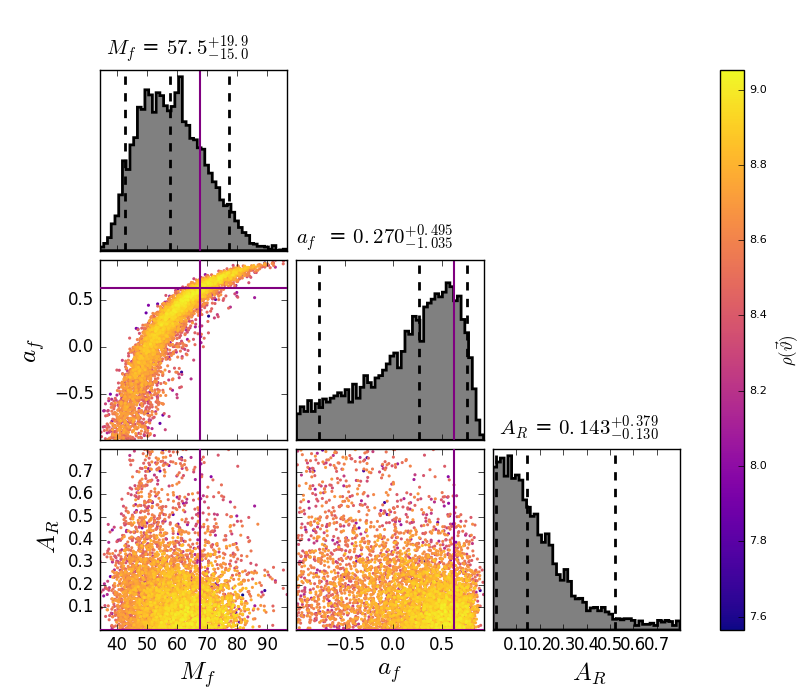
\includegraphics[width=0.5\textwidth]{figures/PE_plot_final/PT_0_pt5_TIMES.png} }
\subfloat{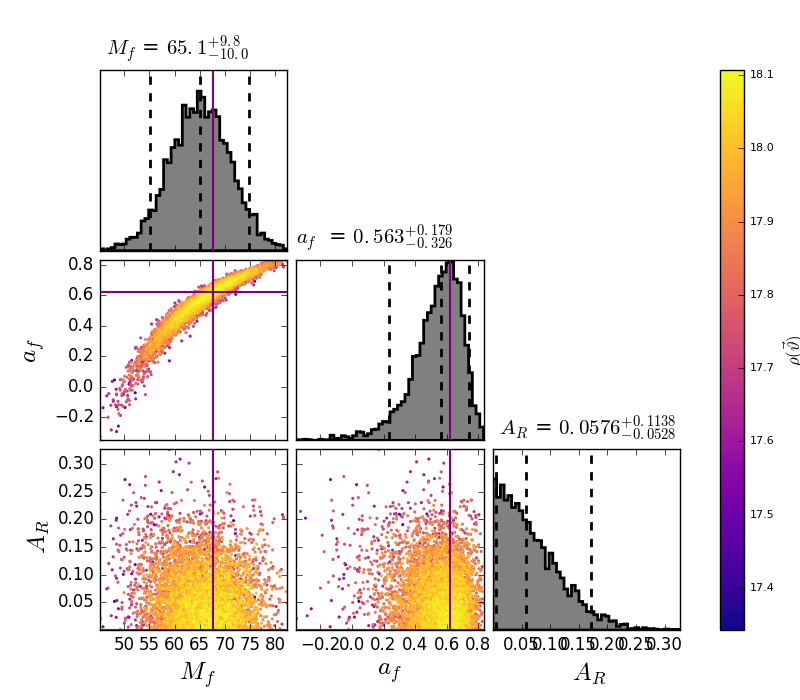
\includegraphics[width=0.5\textwidth]{figures/PE_plot_final/PT_0_1_TIMES.png} }  \\[-0.3cm]
\subfloat{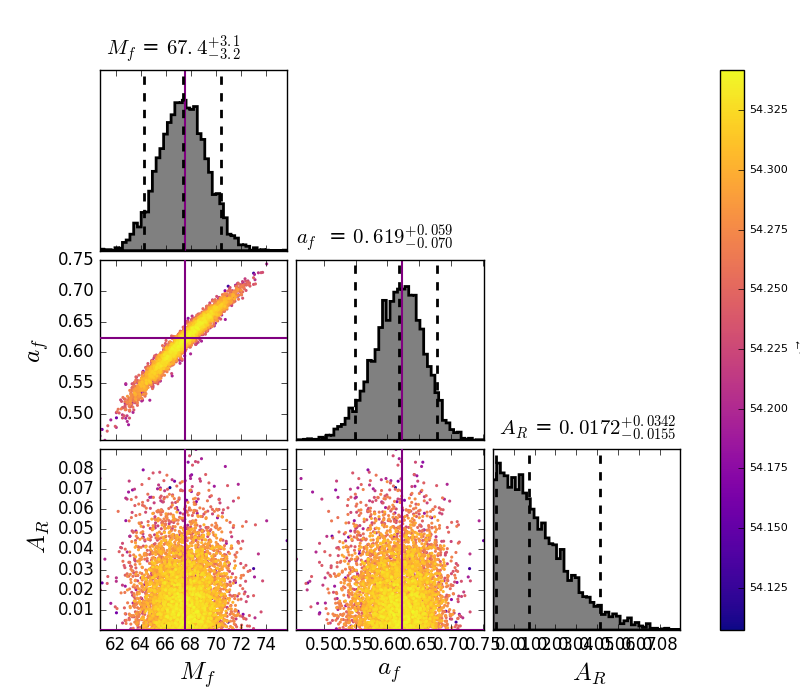
\includegraphics[width=0.5\textwidth]{figures/PE_plot_final/PT_0_3_TIMES.png} }
\subfloat{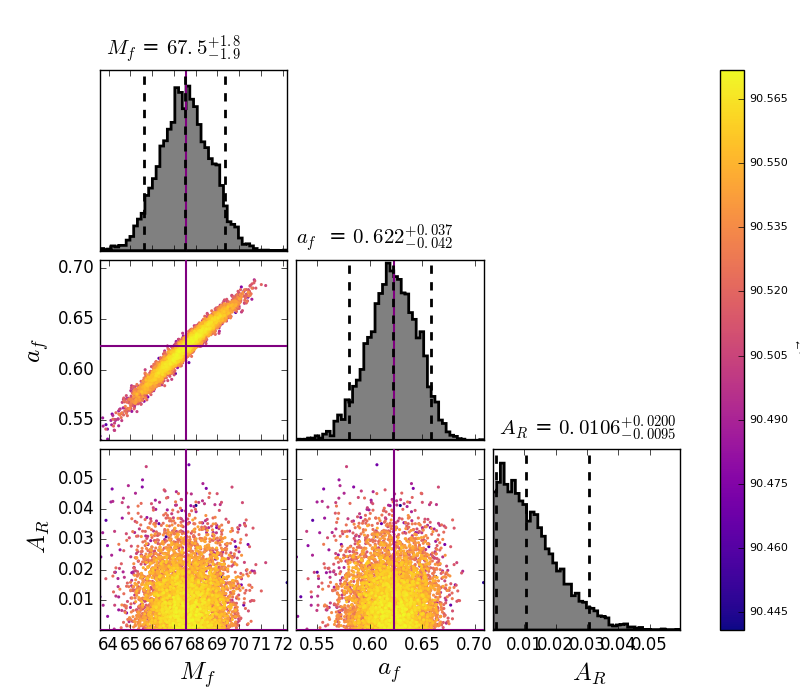
\includegraphics[width=0.5\textwidth]{figures/PE_plot_final/PT_0_5_TIMES.png} }
\caption{PE reults for injections with $A_{R} = 0.0$. This figure shows the result of RD PE performed on an analytical RD injection described in section \ref{sec:details-of-ana-RD} in a zero noise realization. $A_{R} =0$ for all four injection presented in this figure.RD PE is performed using the setup described in section \ref{sec:Implementation}. The purple line in each of these subplot mark the inject value of the parameter. Furthermore, the four panels corresponds to four different loudness of injection and correspond to $\left\lbrace 0.5 A_{0}, A_{0}, 3A_{0}, 5A_{0}\right\rbrace $. The colorbar indicates the recovered SNR. Note that the PE is perfromed over the following set of parameters:  $\left\lbrace  t_{c}, A_{22}, A_{R}, M_{f}, a_{f}, \phi_{22}, \phi_{33 } \right\rbrace $. }  
\label{fig:zero}
\end{figure*}

\begin{figure*}
\subfloat{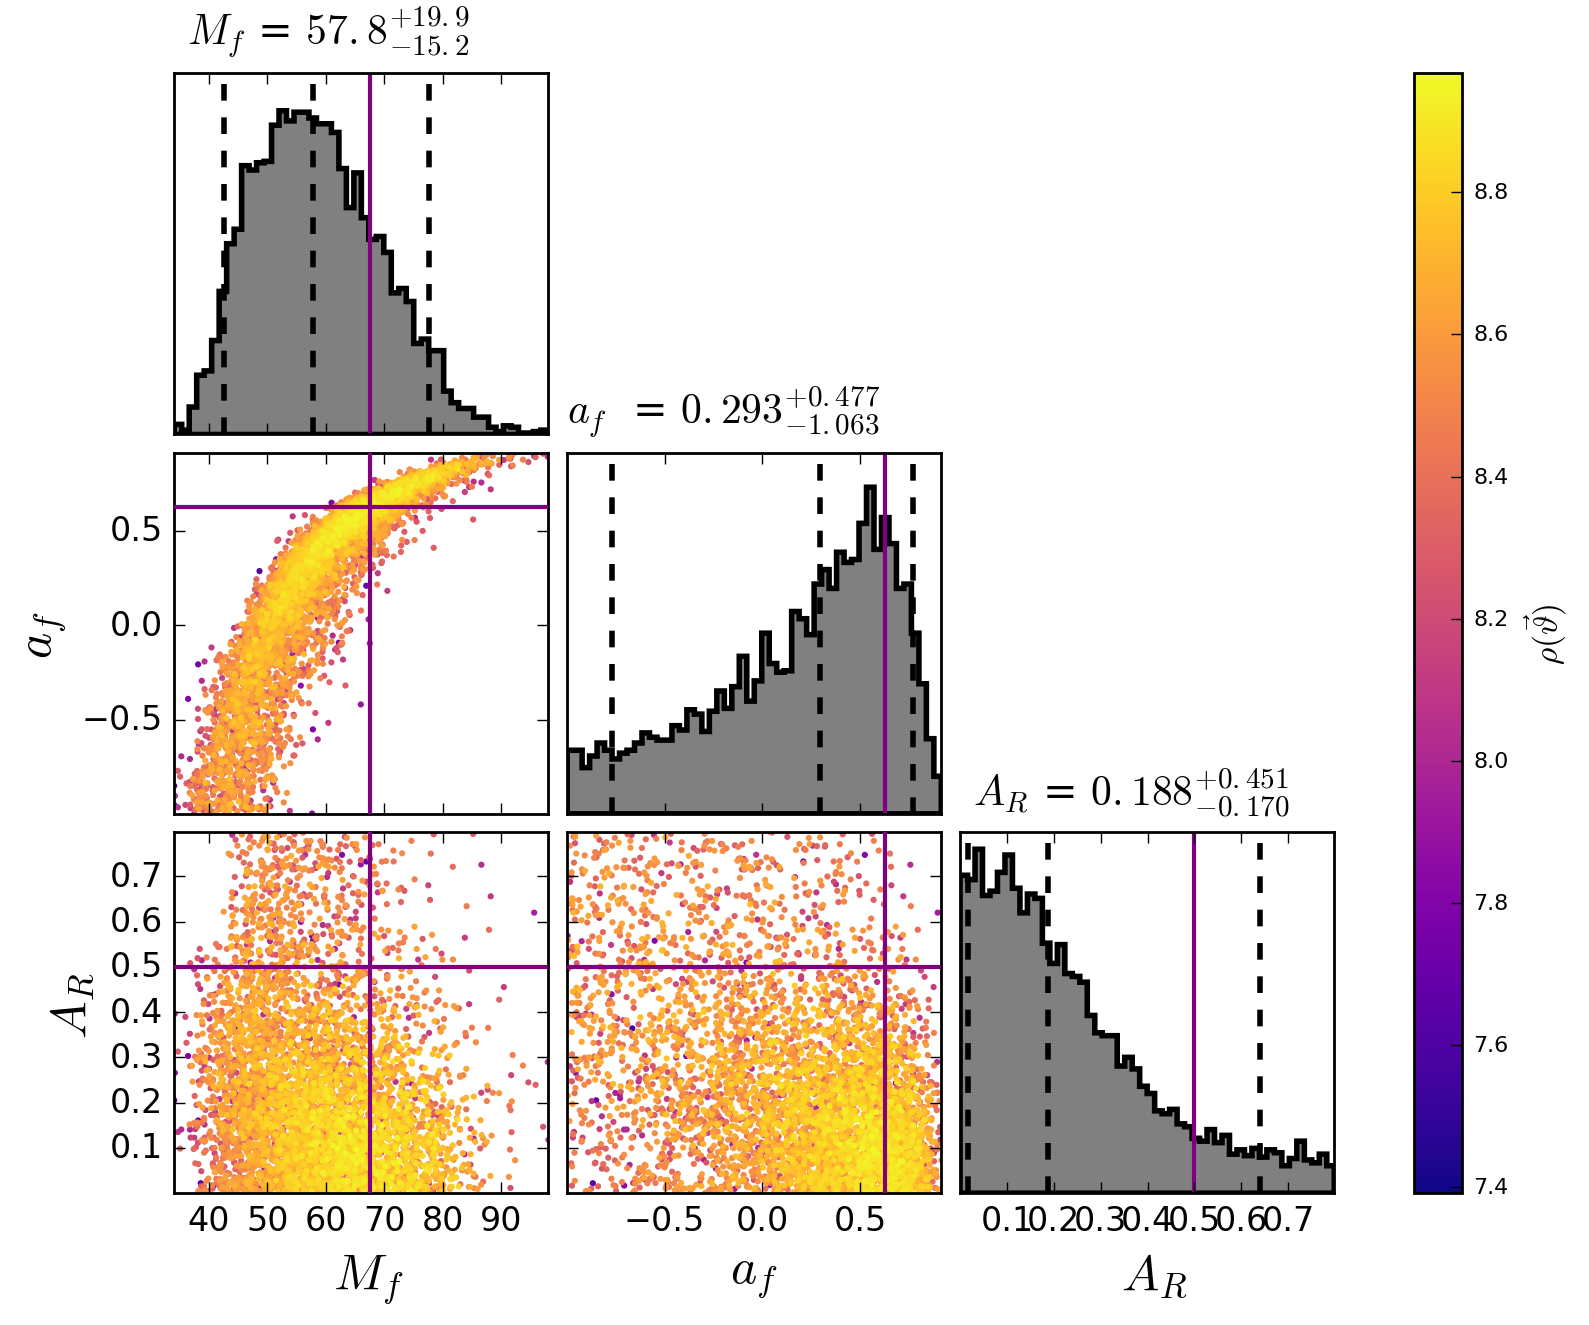
\includegraphics[width=0.5\textwidth]{figures/PE_plot_final/PT_1_pt5_TIMES.png} }
\subfloat{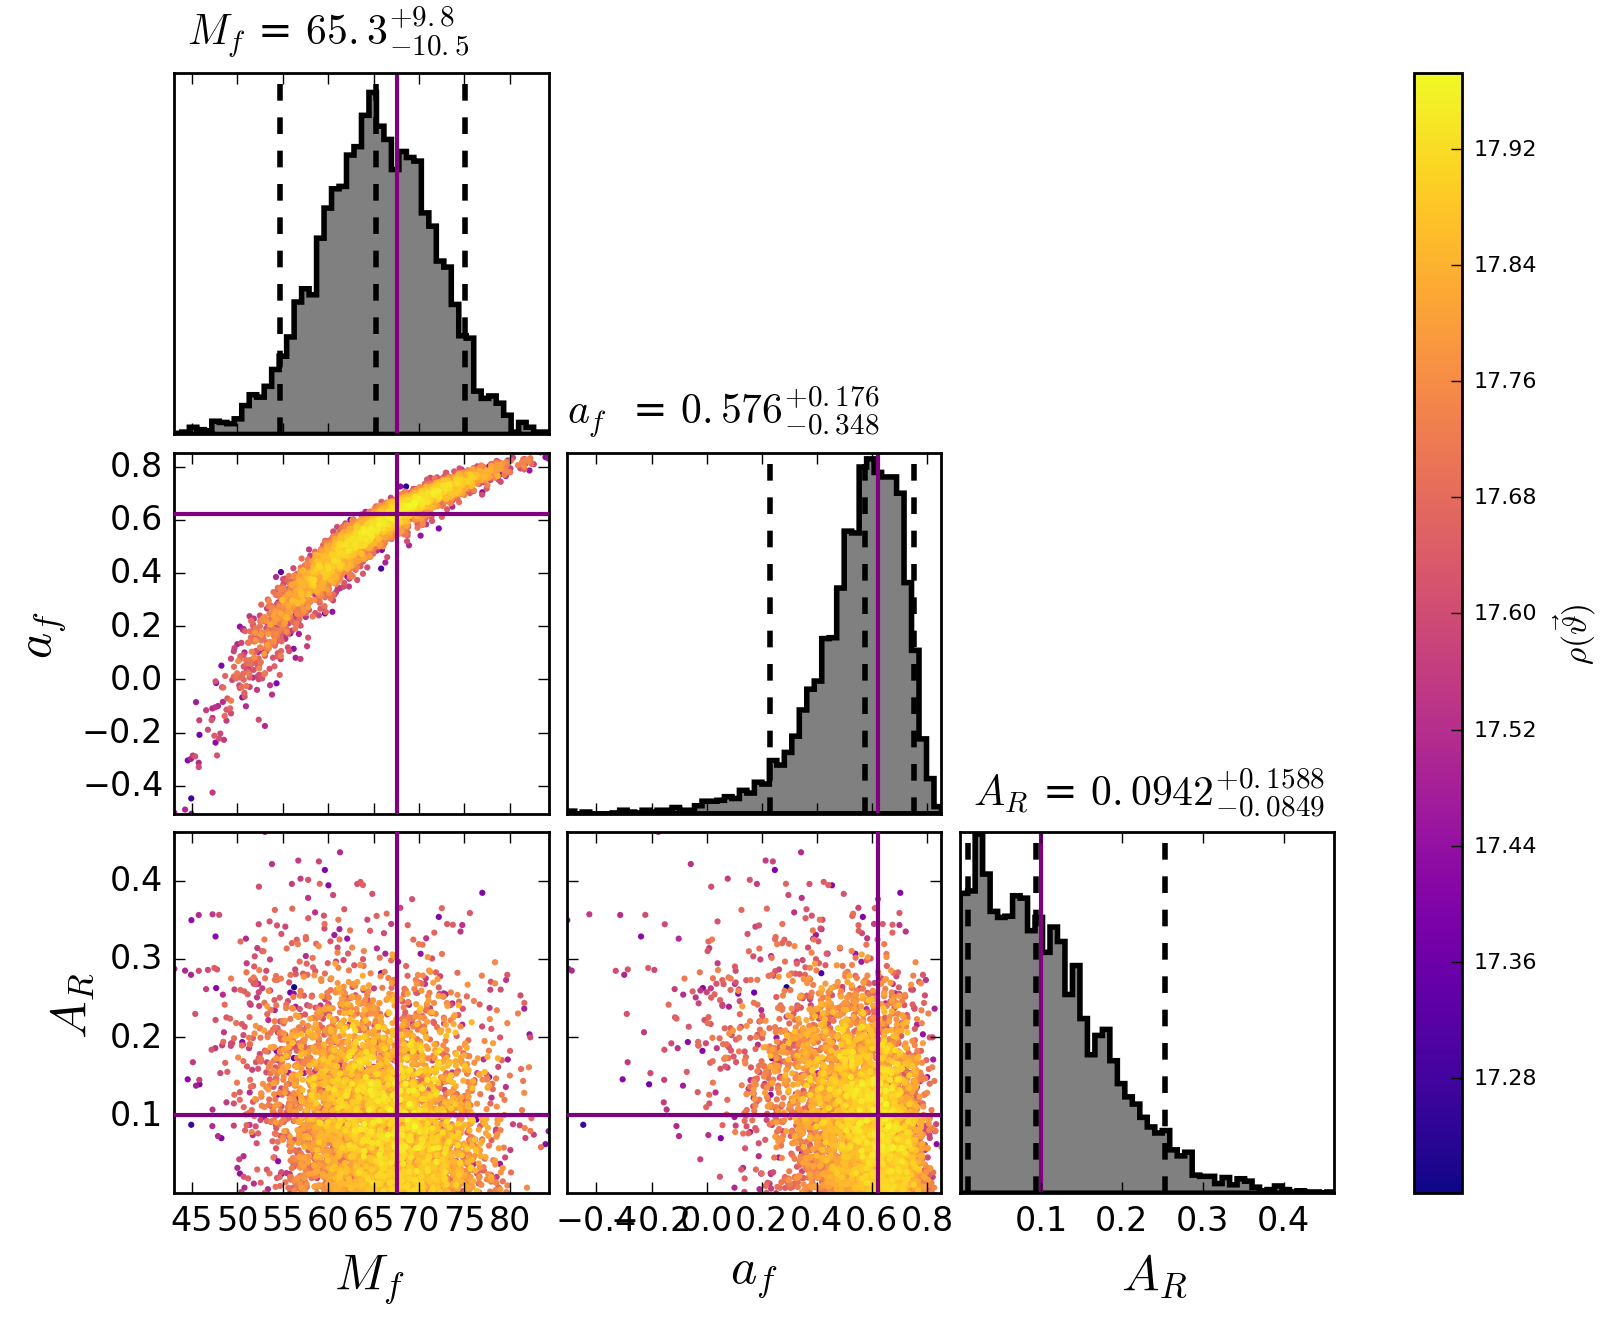
\includegraphics[width=0.5\textwidth]{figures/PE_plot_final/PT_1_1_TIMES.png} }  \\[-0.3cm]
\subfloat{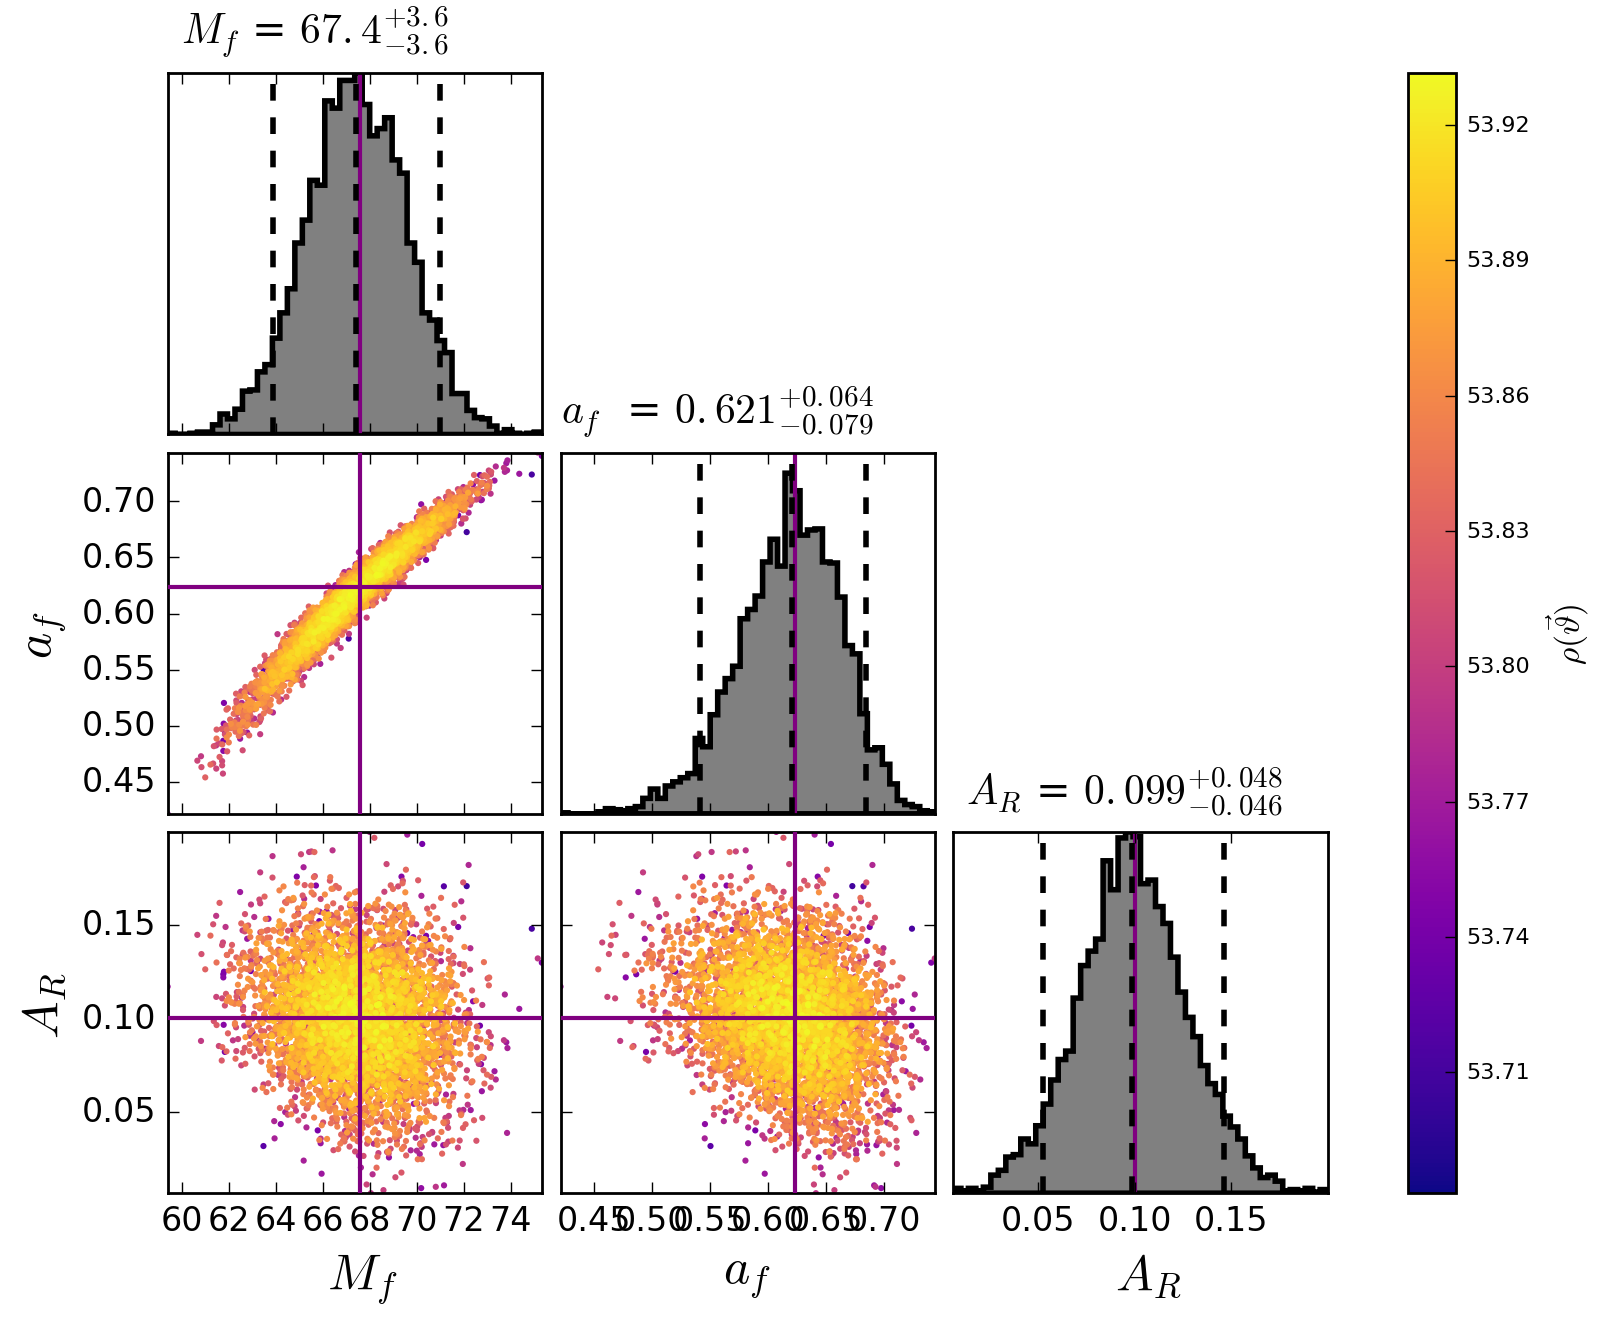
\includegraphics[width=0.5\textwidth]{figures/PE_plot_final/PT_1_3_TIMES.png} }
\subfloat{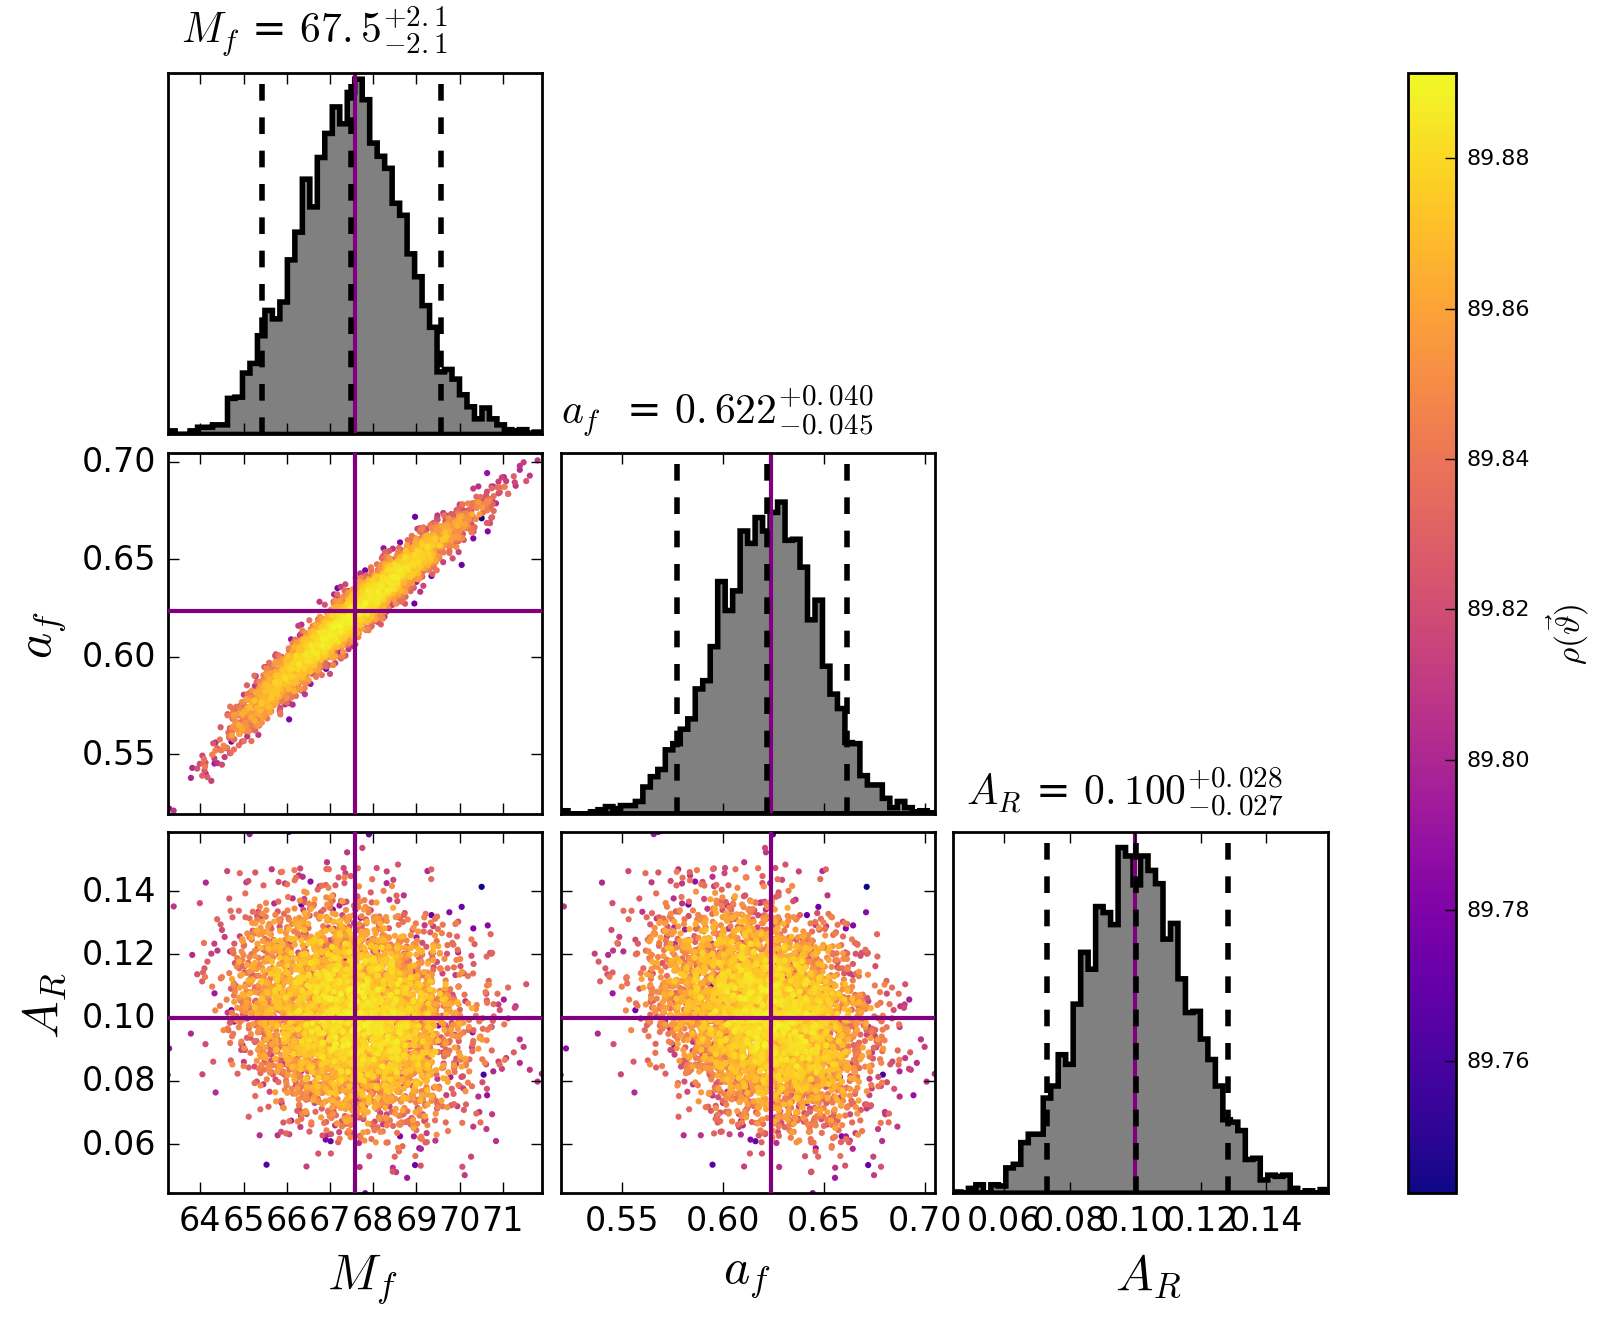
\includegraphics[width=0.5\textwidth]{figures/PE_plot_final/PT_1_5_TIMES.png} }
\caption{PE reults for injections with $A_{R} = 0.1$. This plot is similar to Figure \ref{fig:zero} except for the fact that the mode amplitude ratio $A_{R}=0.1$ }
\label{fig:one}
\end{figure*}

\begin{figure*}
\subfloat{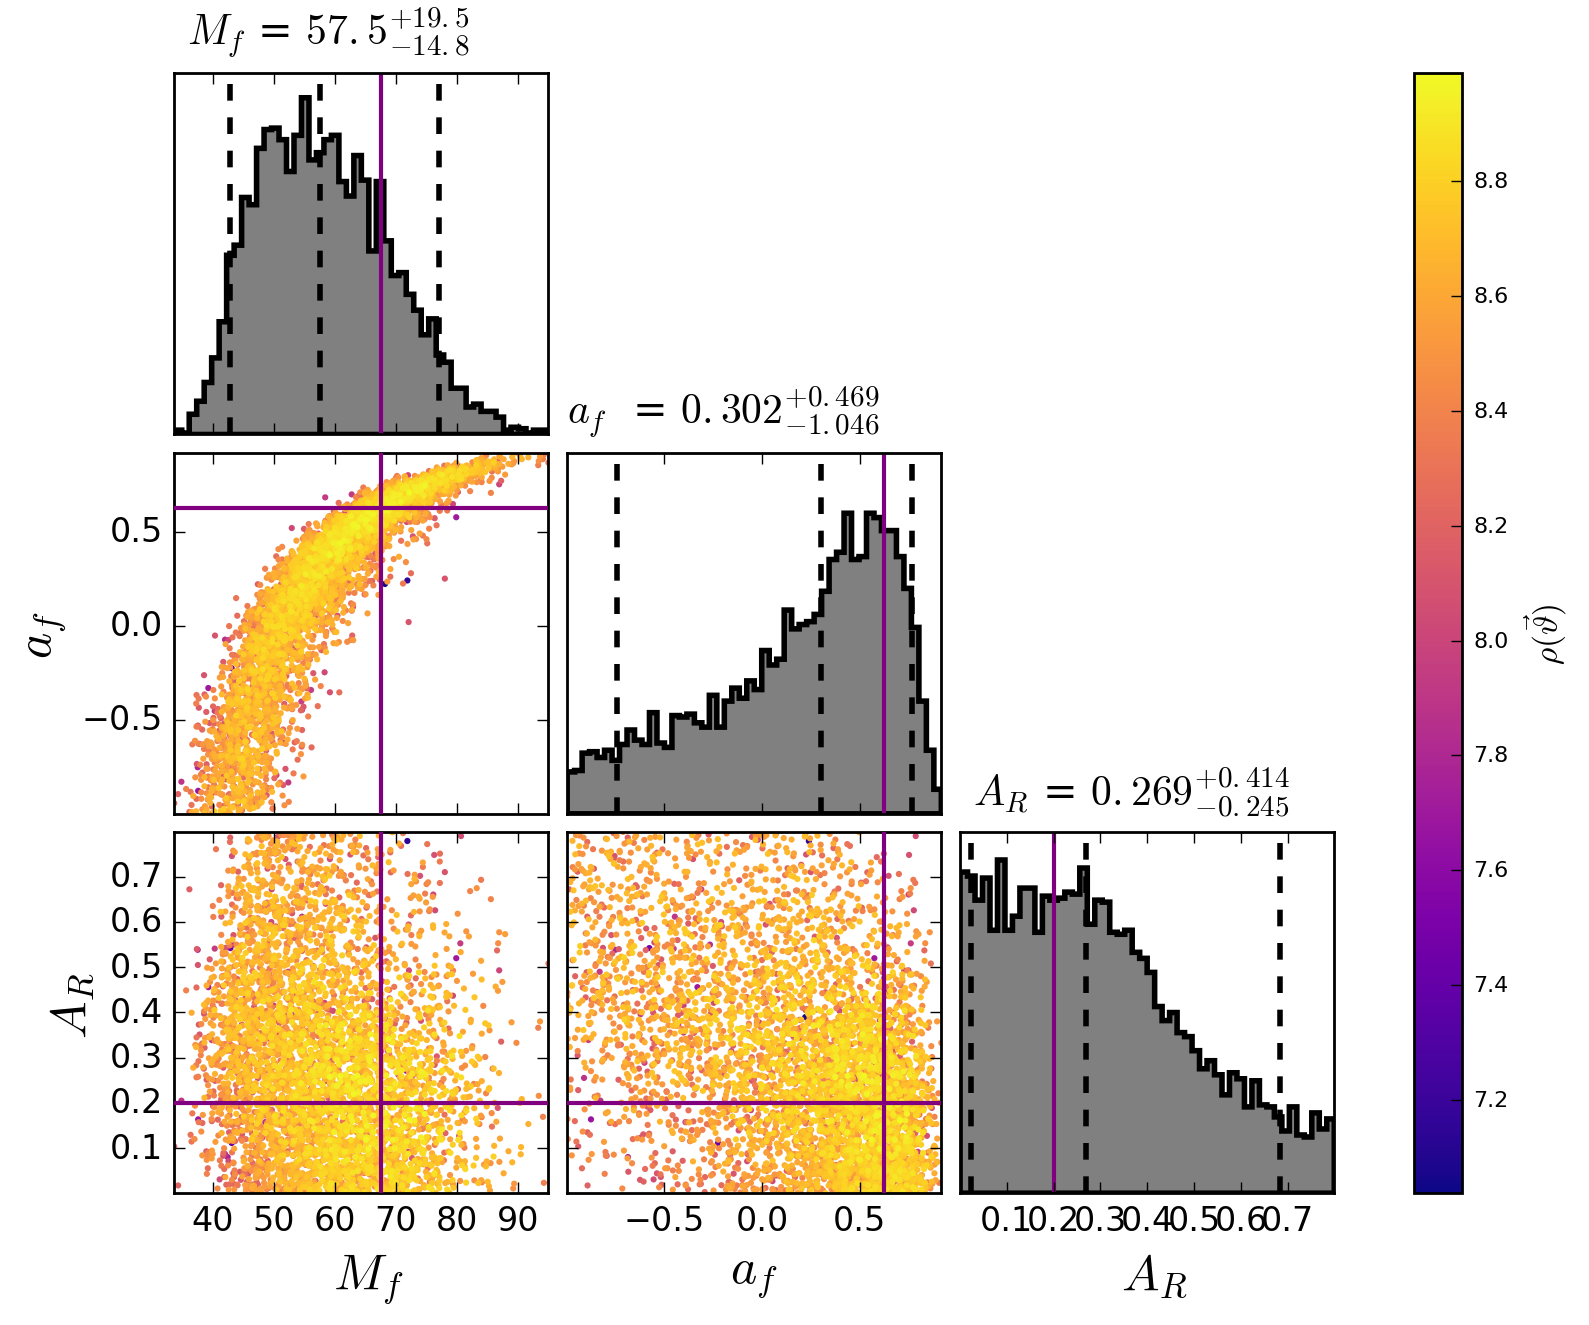
\includegraphics[width=0.5\textwidth]{figures/PE_plot_final/PT_2_pt5_TIMES.png} }
\subfloat{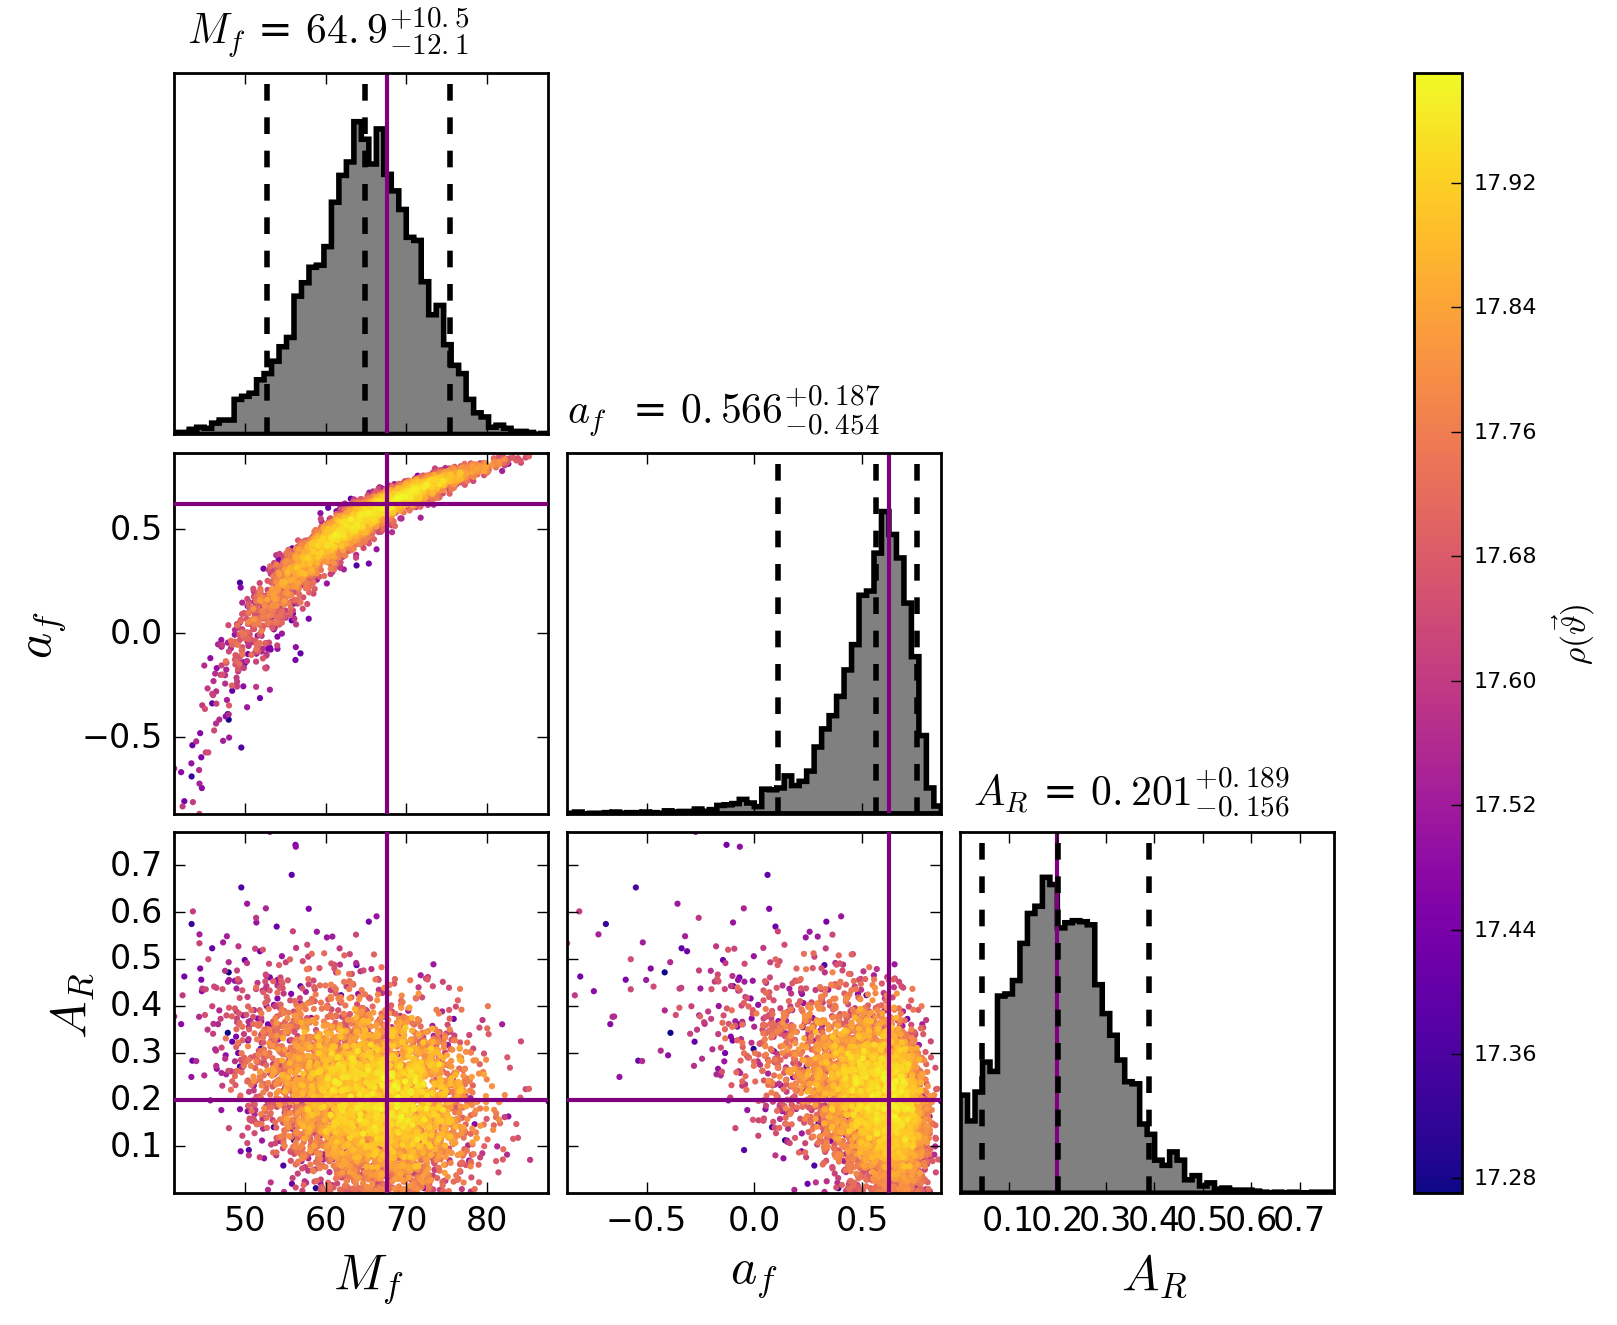
\includegraphics[width=0.5\textwidth]{figures/PE_plot_final/PT_2_1_TIMES.png} }  \\[-0.3cm]
\subfloat{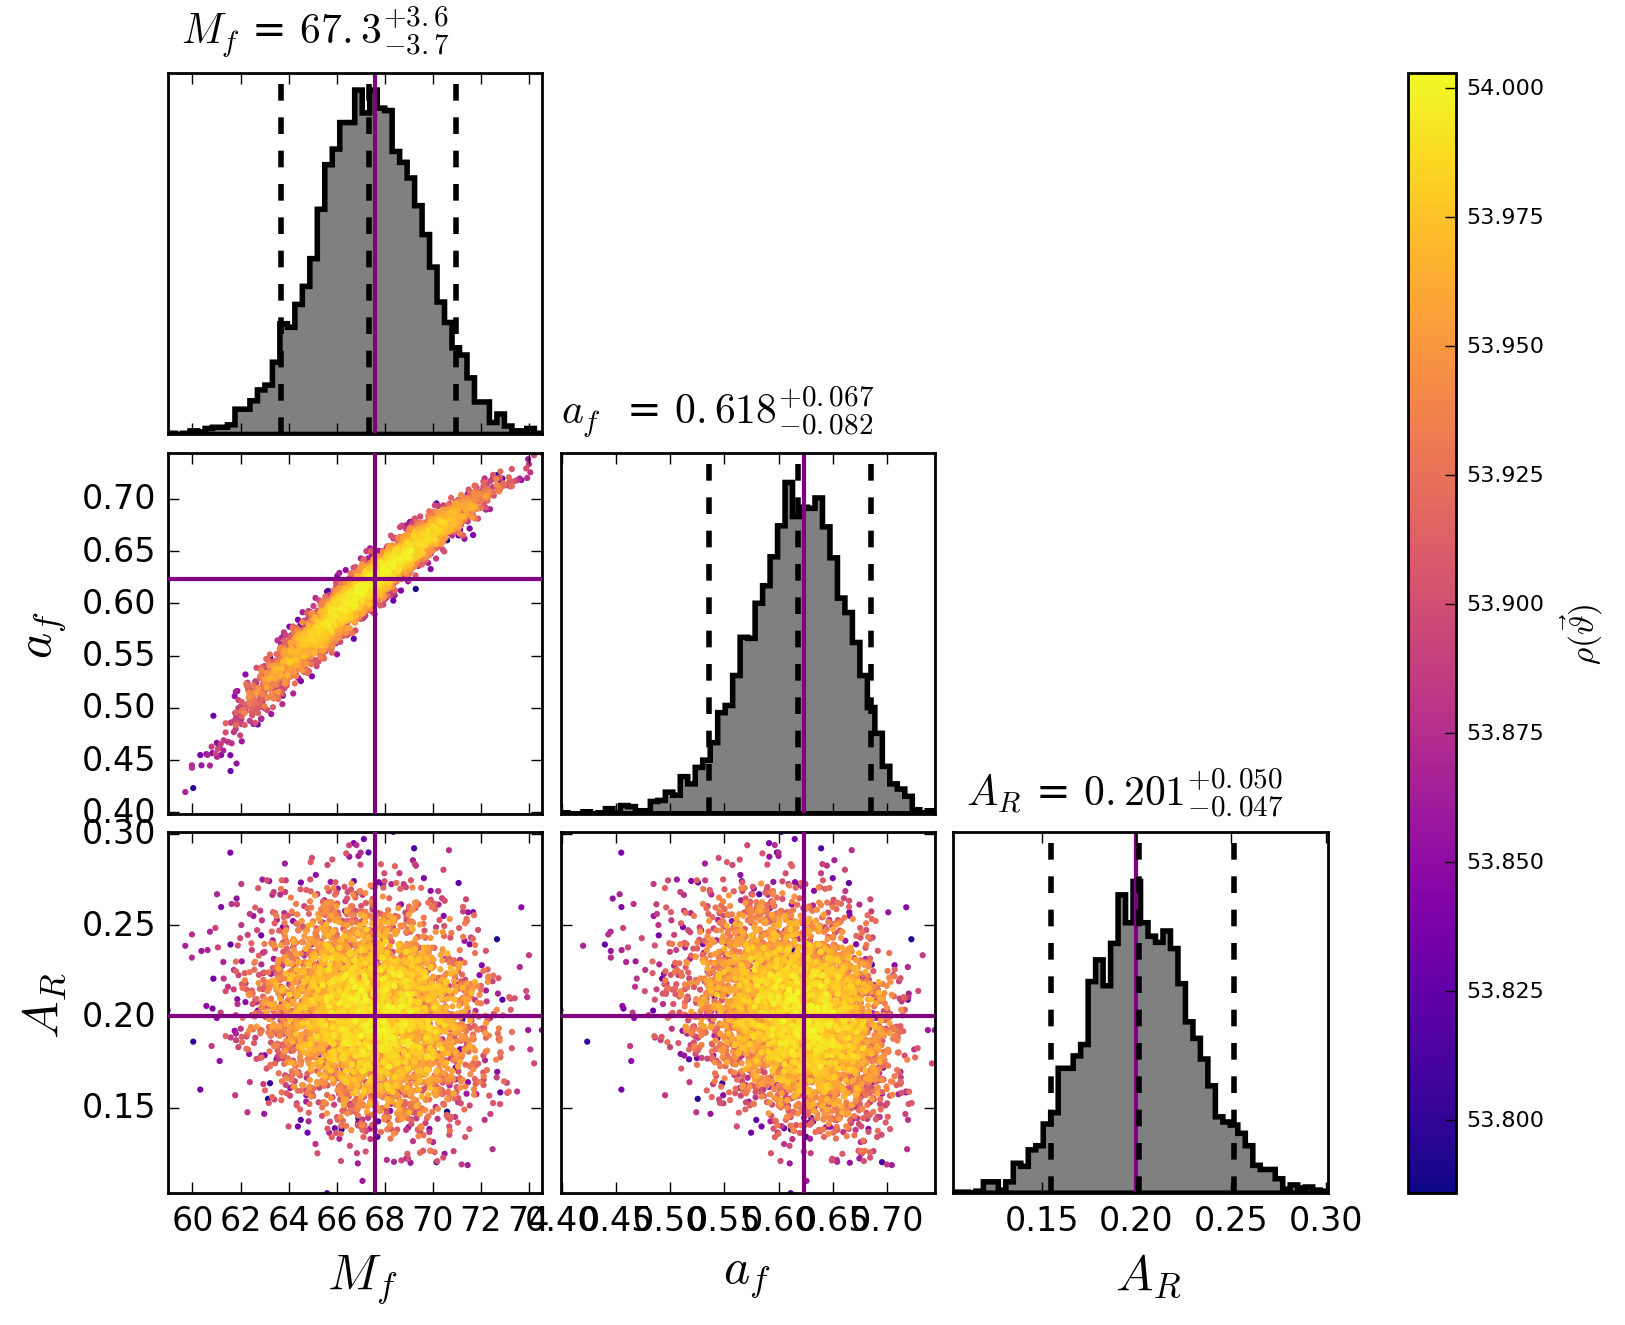
\includegraphics[width=0.5\textwidth]{figures/PE_plot_final/PT_2_3_TIMES.png} }
\subfloat{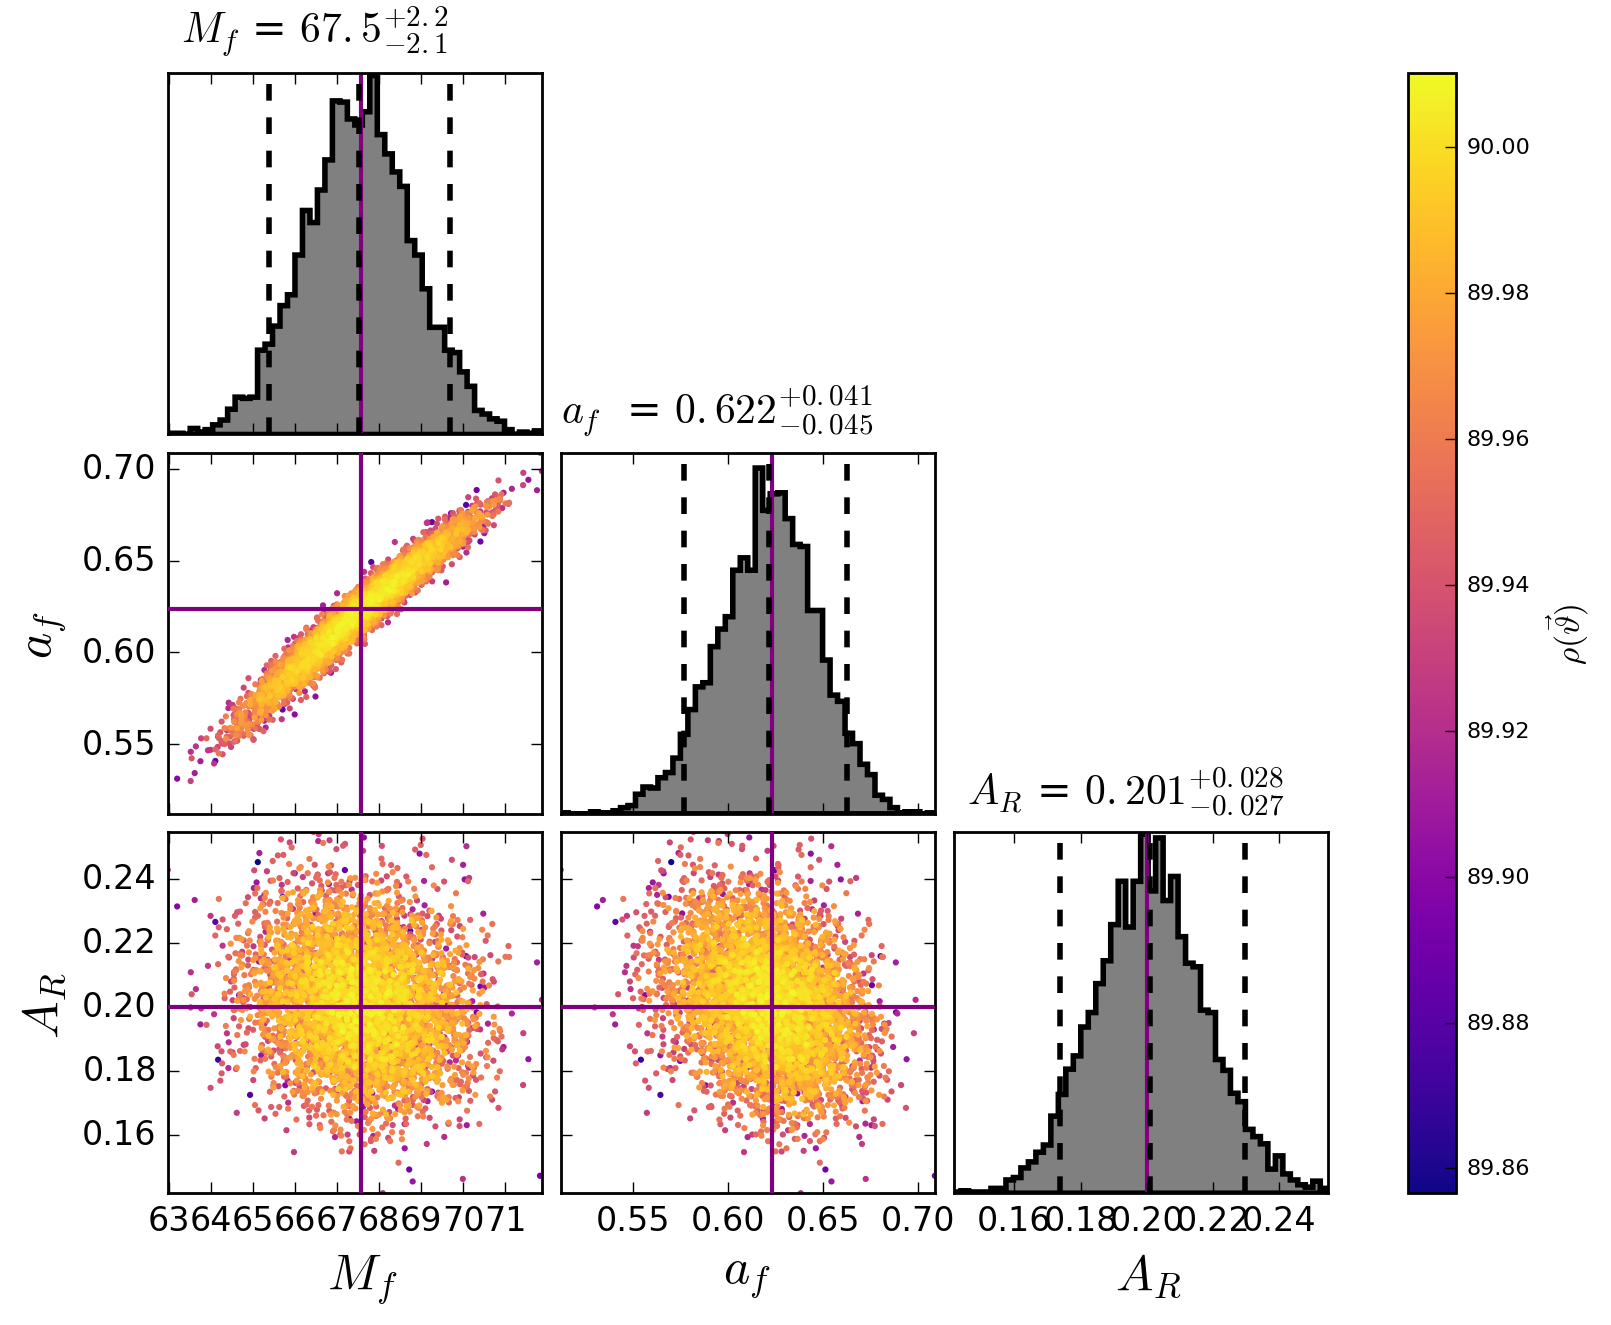
\includegraphics[width=0.5\textwidth]{figures/PE_plot_final/PT_2_5_TIMES.png} }
\caption{PE reults for injections with $A_{R} = 0.2$. This plot is similar to Figure \ref{fig:zero} except for the fact that the mode amplitude ratio $A_{R}=0.2$ }
\label{fig:two}
\end{figure*}

\begin{figure*}
\subfloat{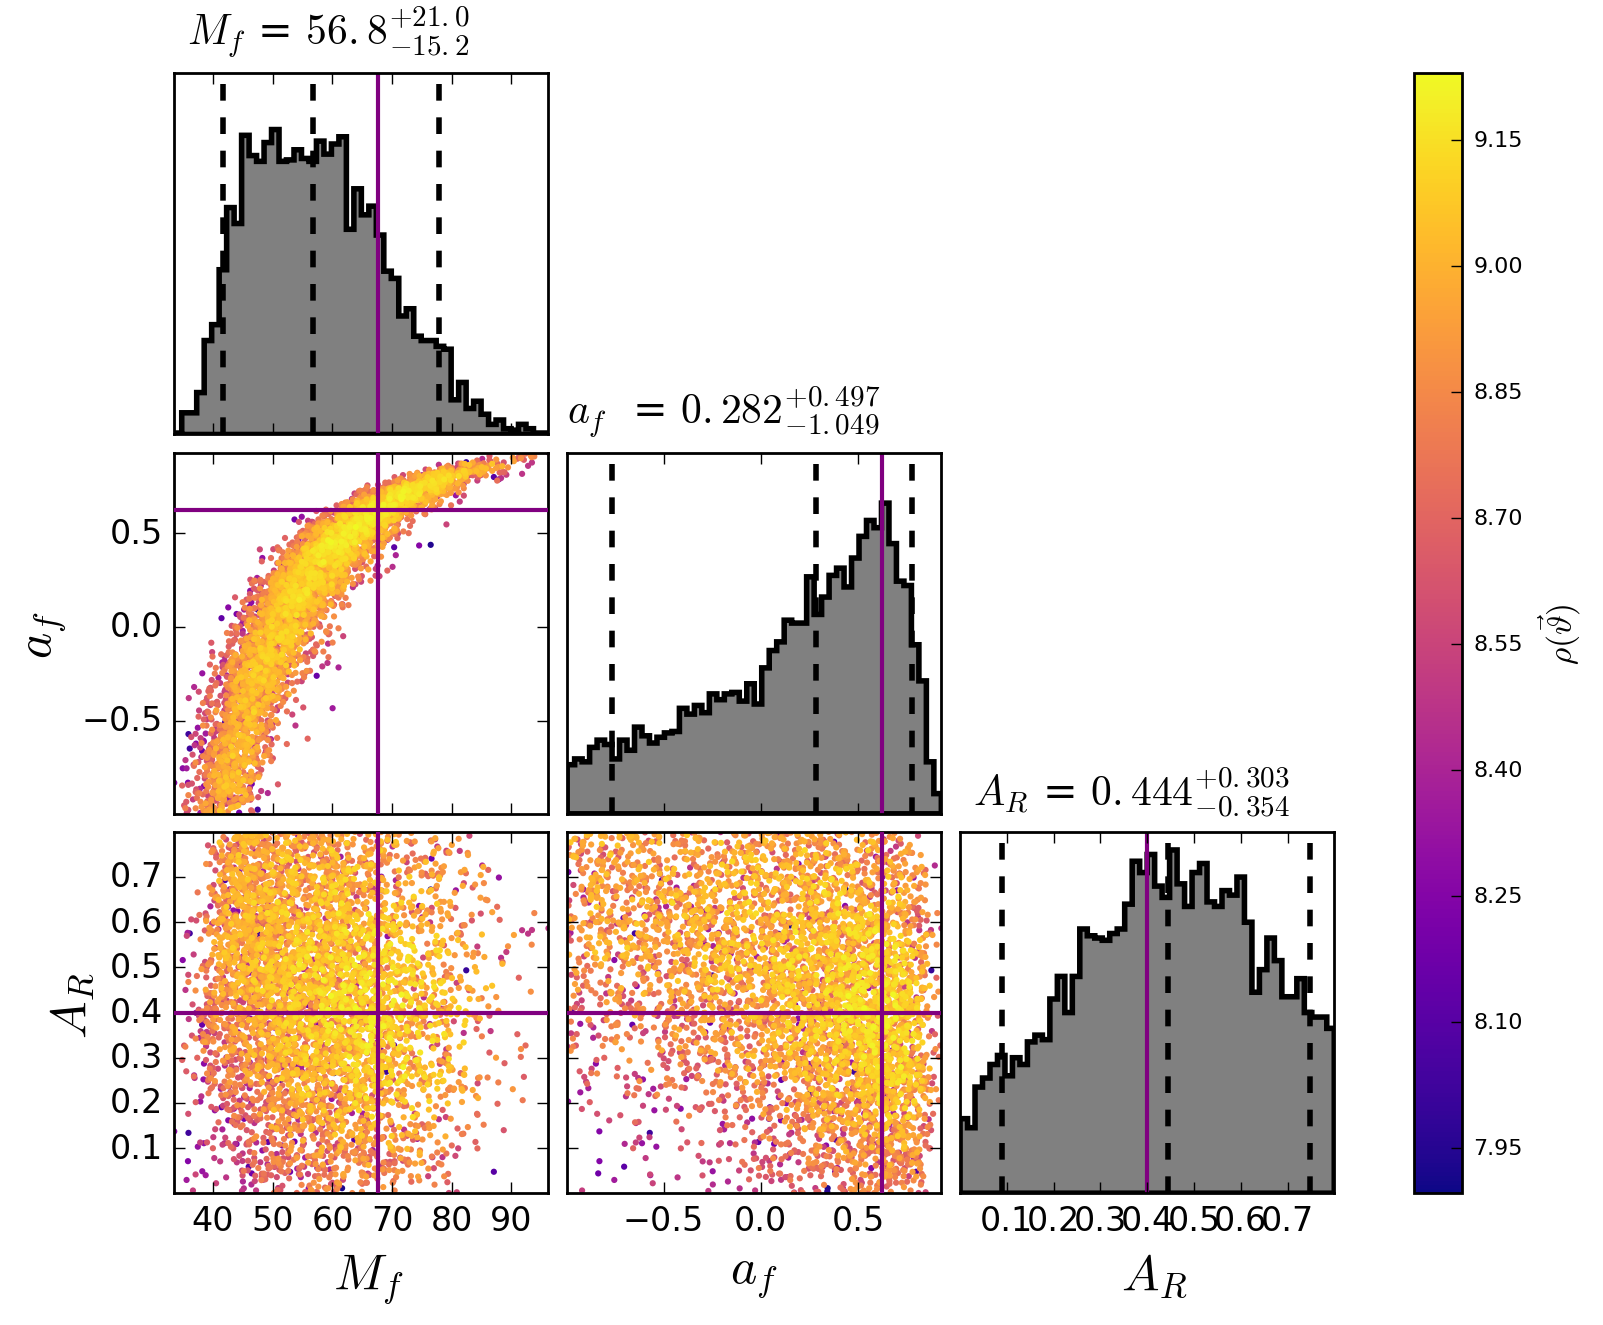
\includegraphics[width=0.5\textwidth]{figures/PE_plot_final/PT_4_pt5_TIMES.png} }
\subfloat{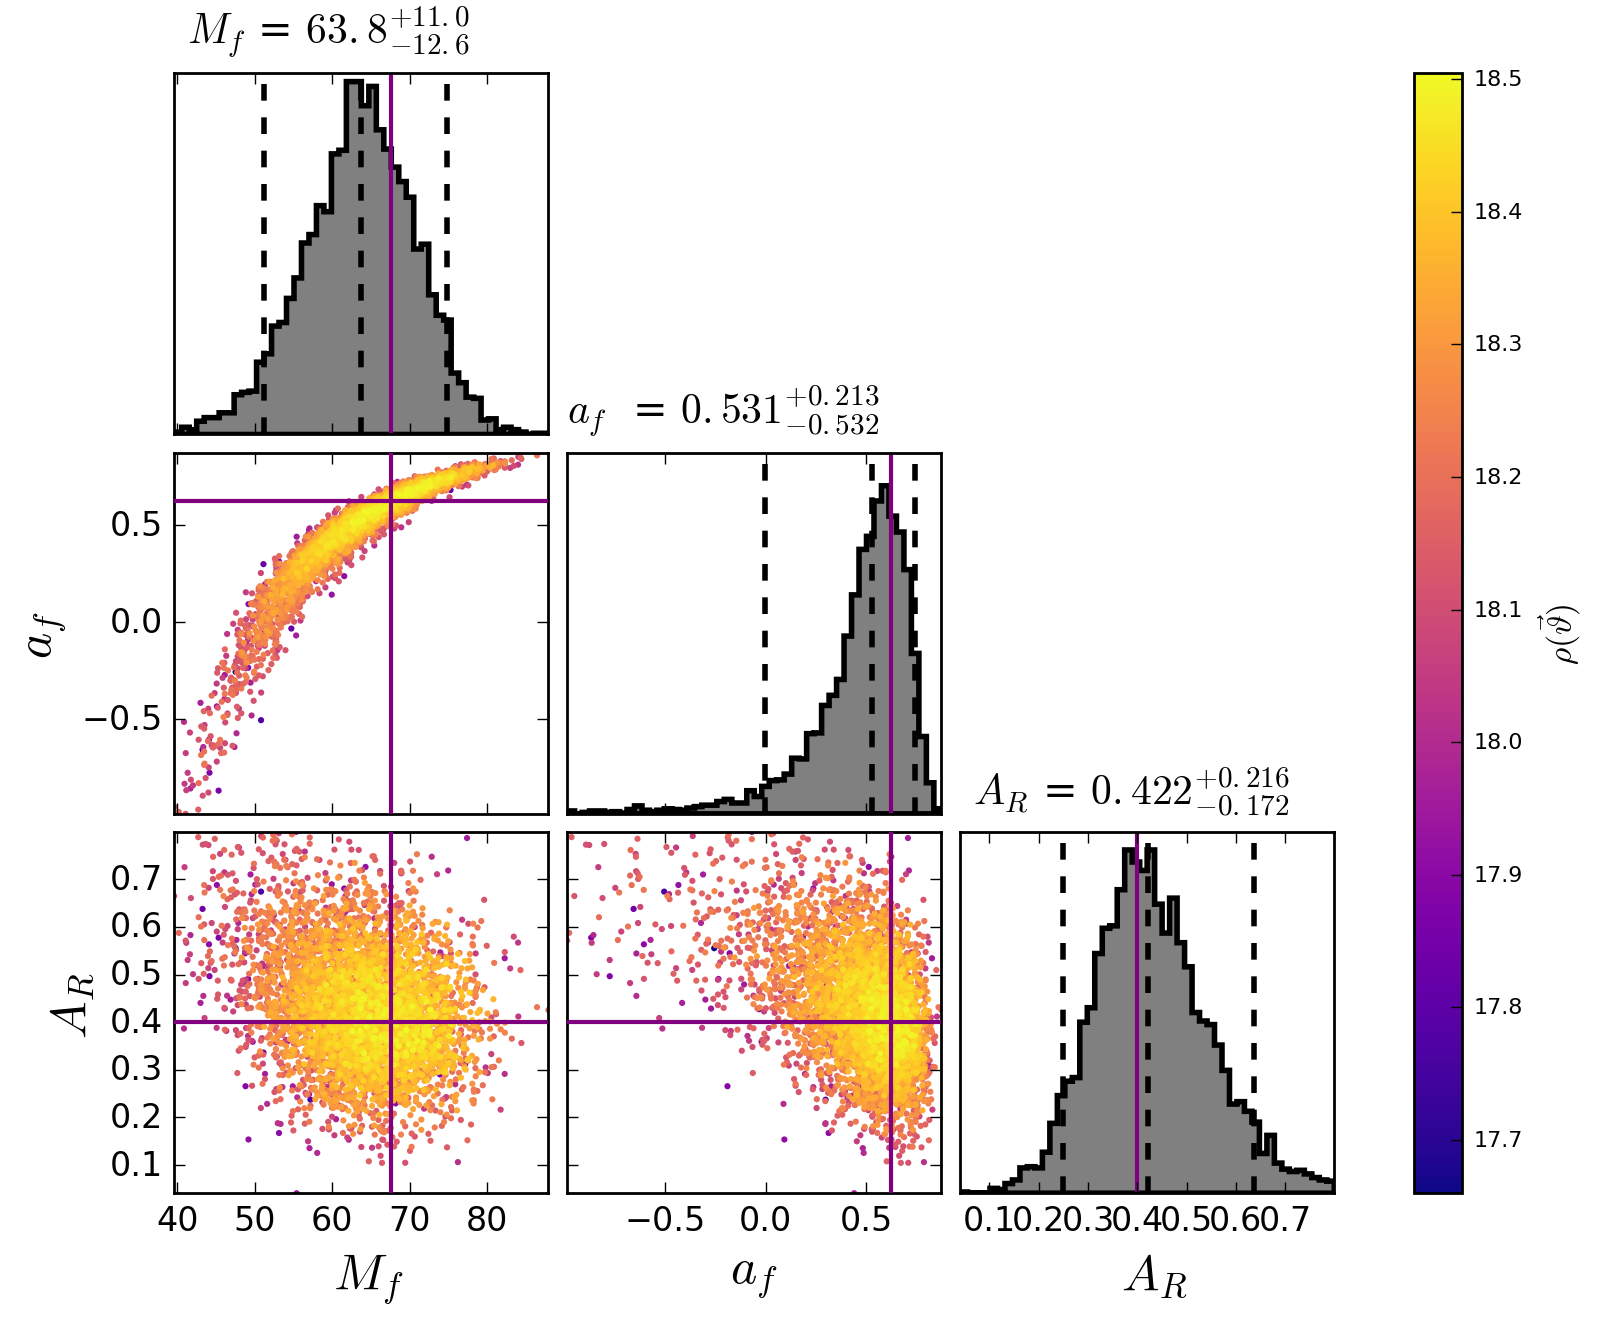
\includegraphics[width=0.5\textwidth]{figures/PE_plot_final/PT_4_1_TIMES.png} }  \\[-0.3cm]
\subfloat{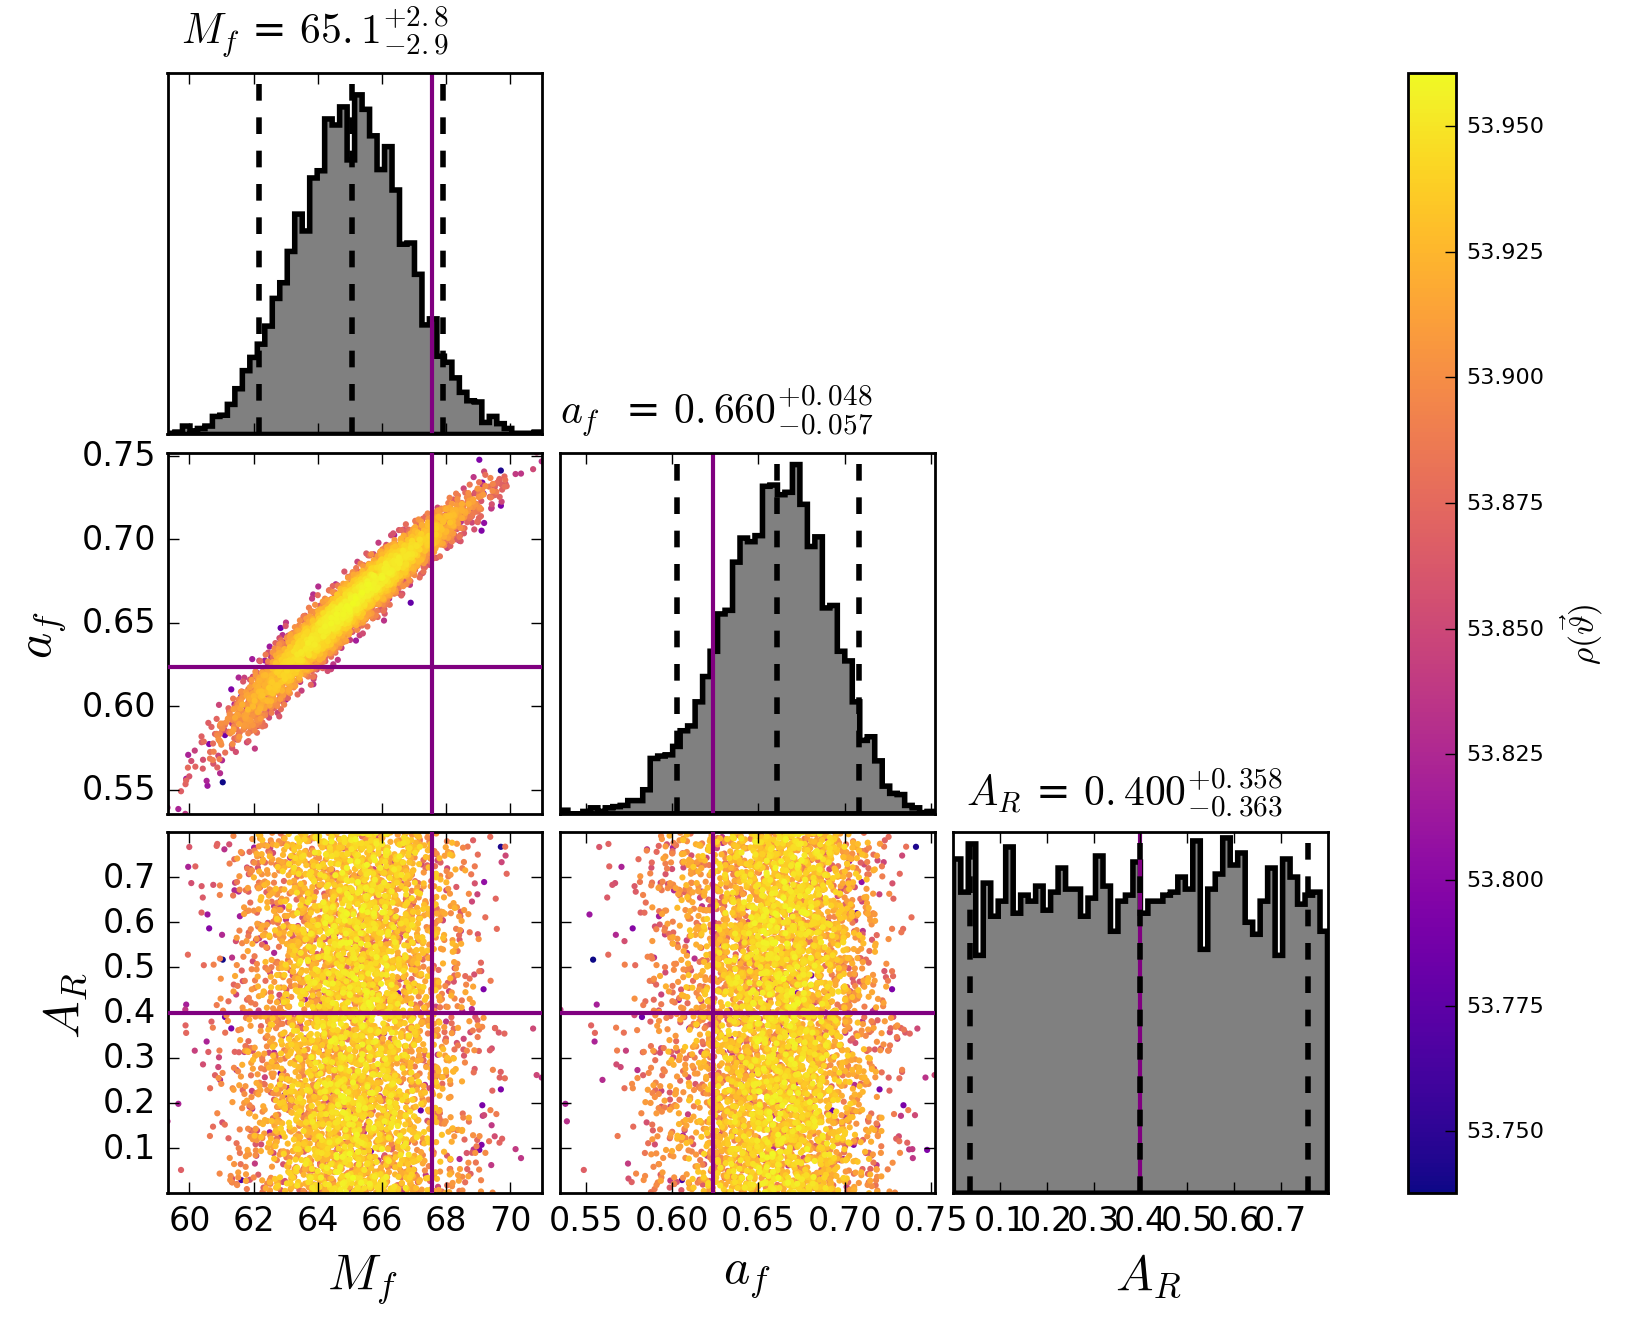
\includegraphics[width=0.5\textwidth]{figures/PE_plot_final/PT_4_3_TIMES.png} }
\subfloat{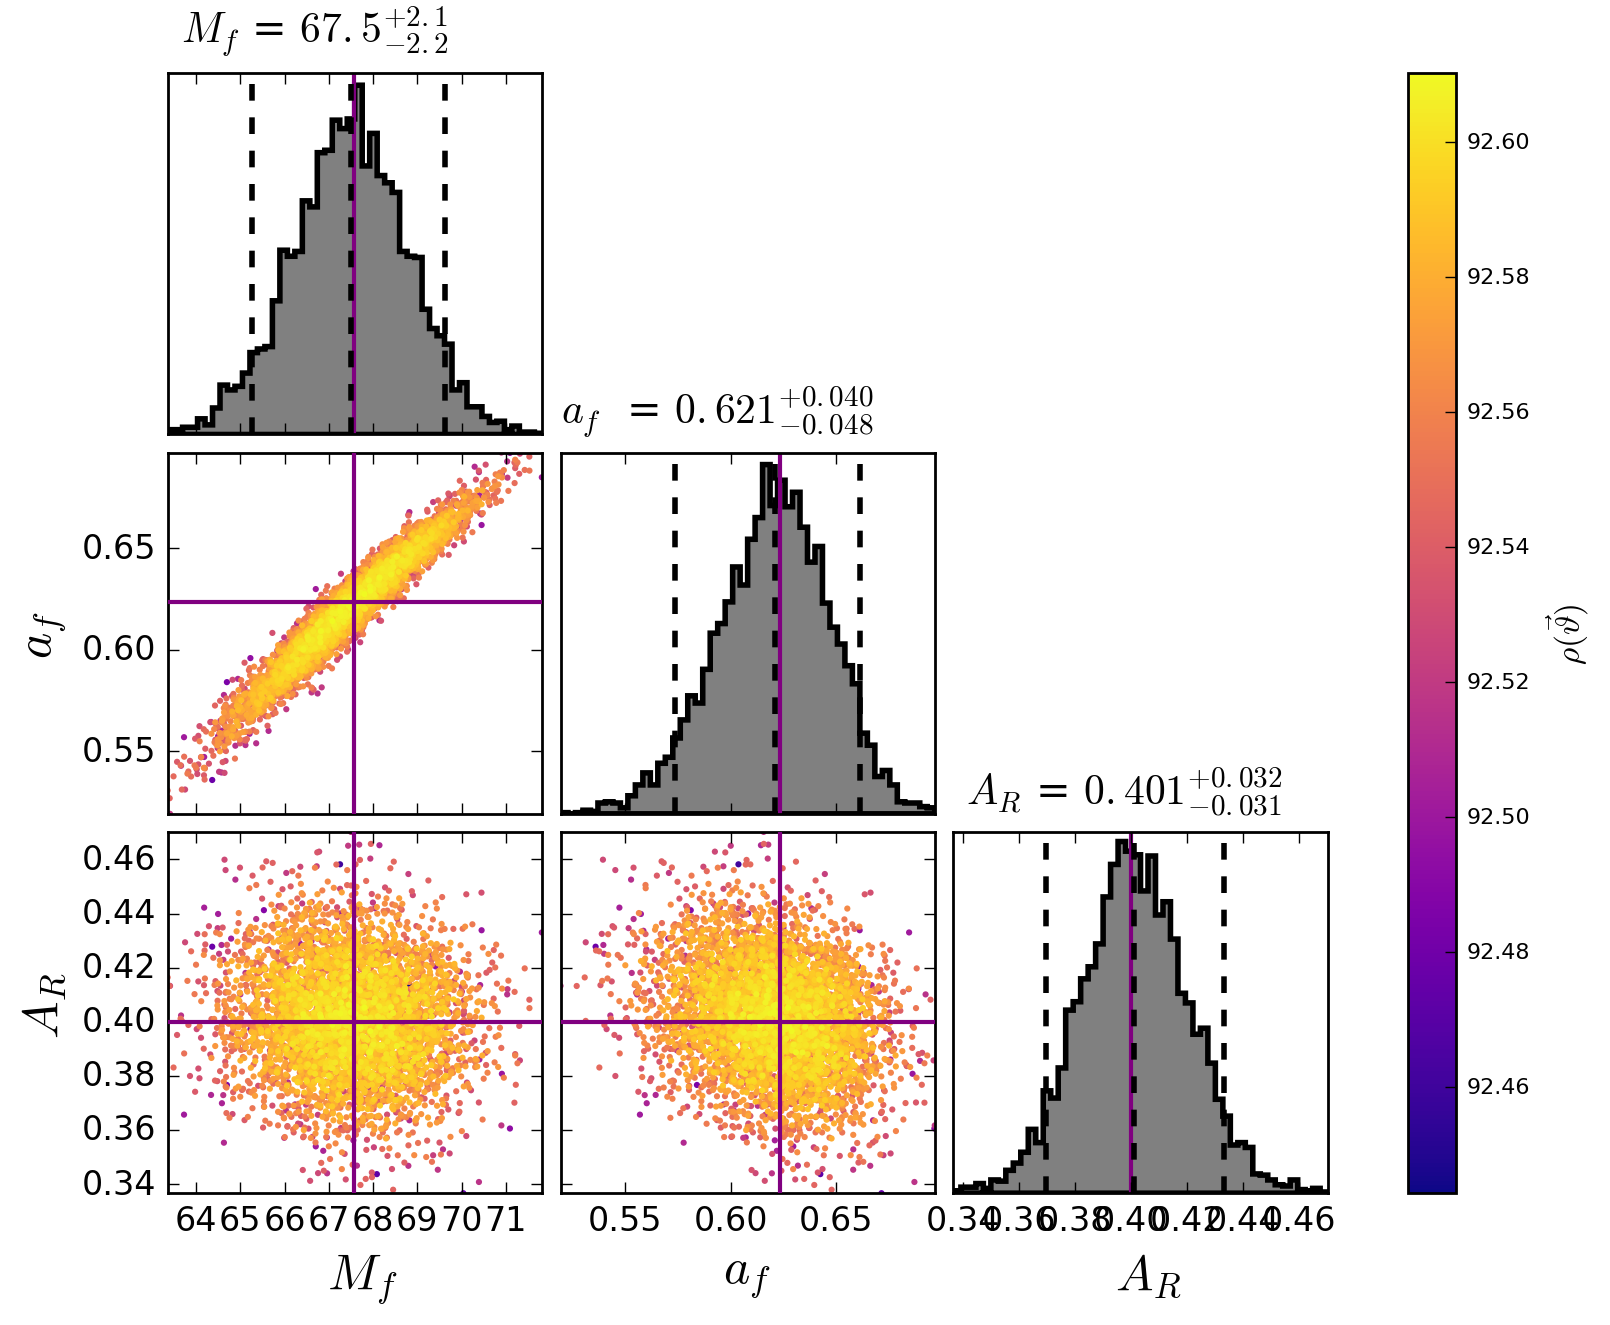
\includegraphics[width=0.5\textwidth]{figures/PE_plot_final/PT_4_5_TIMES.png} }
\caption{PE reults for injections with $A_{R} = 0.4$. This plot is similar to Figure \ref{fig:zero} except for the fact that the mode amplitude ratio $A_{R}=0.4$ }
\label{fig:four}
\end{figure*}


The results obtained on performing PE using the set up descibed in section \ref{sec:Implementation} on the injection set presented in section \ref{sec:details-of-ana-RD} are showed in Figures \ref{fig:zero}, \ref{fig:one}, \ref{fig:two}, \ref{fig:four}. Figure \ref{fig:zero} is a null test, where is singal comprises of only the dominant mode, i.e. $A_{R}^{\mathrm{Injected}}=0$. Figures \ref{fig:one,fig:two,fig:four} contain injection with $A_{R}^{\mathrm{Injected}}$ set  0.1, 0.2
 and 0.4 respectively. The panels in each of these figures correspond to four amplitudes of the $l=m=2$ mode $A_{22}$ that we choose to investigate-  $\left\lbrace 0.5 A_{0}, A_{0}, 3A_{0}, 5A_{0}\right\rbrace $. The question that we try to address with this study is detactability of the subdominant mode in RD. In the context of this study, when the 90\% credible interval of posterior distribution of $A_{R}$ estimated from the data excludes $A_{R} = 0$, we infer the presence of subdominant mode.  

Note that for the null test, i.e. $A_{R}^{\mathrm{Injected}} =0$, presented in Figure \ref{fig:zero}, the distribution of the estimated value of $A_{R}$ peaks around zero for all values of $A_{22}$ that we study.  Furthermore, the estimated values of $ \left\lbrace M_{f},  a_{f} \right\rbrace$ in each of these cases are consistent with the injected value. Furthermore, in each of the figures \ref{fig:zero, fig:one, fig:two, fig:four}, we see that as we increase the value of injected $A_{22}$, the maximum a posteriori estimate (MAP) value of all the parameters converges to the true injected value. 

Comparing the figures \ref{fig:zero}, \ref{fig:one}, \ref{fig:two}, \ref{fig:four}, we find that for a given SNR, detectability of the sub-dominant mode depends strongly on the injected value of $A_{R}$. For instance, consider a PE performed on a signal with an SNR $\sim 18$ in ringdown but with varying amplitude ratio $A_{R}$. The results of PE done on four such systems are presented in the top right panel of Figures \ref{fig:zero, fig:one, fig:two, fig:four}.  The 90 \% credible interval of the estimated parameter $A_{R}$ has a support for $A_{R} =0$ when $A_{R}^{\mathrm{Injected}} = 0.1$. Therefore, in this case, we cannot confirm the presence of the subdominant mode in the framework of our study. Although its presence cannot be detected by our criterion, we would like to emphasise that comparing the top right panels of Figure ref{fig:zero, fig:one} one can see that for the case of $A_{R}^{\mathrm{Injected}} = 0.1$ the distribution is slightly shifted away from $A_{R}=0$. Therefore, a more refined analysis like a Bayesian model selection between one-mode and two-mode template models might allow us to infer the presence of the sub-dominant mode in this case. We plan to implement a Bayesian model selection scheme to investigate this in near future.  

When $A_{R}^{\mathrm{Injected}} = \left\lbrace 0.2, 0.4 \right\rbrace $, from top right panels of Figures \ref{ fig:two, fig:four}, we see that the 90 \% credible interval of the estimated parameter $A_{R}$ excludes $A_{R} =0 $. Therefore, in these cases, we can infer the presence of the subdominant mode in the ringdown. Moreover, it must be highlighted that the posterior distribution for $A_{R}$ peaks close to the true injected value $A_{R} $, i.e. MAP estimate of $A_{R}$ is consistent with the true injected value.   

From table 2 of \cite{bertiparam}, we would like to stress on the fact that $A_{R} =0.2 $ corresponds to a progenitor BBH system with mass ratio slightly greater than 2. This is realistically plausible astrophysical signal that can be observed by LIGO in its future runs. Furthermore, the SNR in the ringdown of GW150914 was $\sim 8$ and it is promising to see that at an SNR $\sim 18$, we begin detecting the presence of the sub-dominant modes in ringdown. This is especially encouraging because the advanced LIGO at its design sensitivity is expected to be about three times as sensitive as it was when we detected GW150914. 

  


